\pdftrailerid{}
\documentclass[11pt]{article}
\usepackage[T1]{fontenc}
\usepackage{lmodern}
\usepackage[letterpaper,margin=1in,headheight=15pt]{geometry}
\usepackage{amsmath,amssymb,amsthm}
\usepackage{microtype,booktabs,array,enumitem,graphicx,longtable}
\usepackage{xcolor,tikz}
\usetikzlibrary{arrows.meta,positioning}
\usepackage{fancyhdr}
\usepackage[colorlinks=true,linkcolor=blue!40!black,urlcolor=blue!40!black,citecolor=blue!40!black]{hyperref}
% Added 4 October 2026, batch 91O: let long file paths break at _ and -.
\makeatletter\g@addto@macro\UrlBreaks{\do\_\do\-}\makeatother
\setlength{\emergencystretch}{2em}
\hypersetup{pdftitle={Zero auxiliary clipping tables and A196460: exact counts, all orders asymptotics, and sharp uniform finite sector truncations},pdfauthor={},pdfsubject={Merged report a196460-clipping-tables (batch 91O): exact classification, counting, fixed-order and uniform asymptotics, and threshold inversion}}
\pagestyle{fancy}
\fancyhf{}
\fancyhead[L]{\small Zero auxiliary clipping tables}
\fancyhead[R]{\small A196460}
\fancyfoot[C]{\thepage}
\renewcommand{\headrulewidth}{0.3pt}
\setlength{\parskip}{4pt}
\setlength{\parindent}{1.25em}
\setlist{topsep=4pt,itemsep=2pt}
\allowdisplaybreaks[1]
\newtheorem{theorem}{Theorem}[section]
\newtheorem{lemma}[theorem]{Lemma}
\newtheorem{proposition}[theorem]{Proposition}
\newtheorem{corollary}[theorem]{Corollary}
\theoremstyle{definition}
\newtheorem{definition}[theorem]{Definition}
\theoremstyle{remark}
\newtheorem{remark}[theorem]{Remark}
\newcommand{\Npos}{\mathbb Z_{>0}}
\newcommand{\E}{\mathbb E}
\newcommand{\Z}{\mathbb Z}
\newcommand{\la}{\lambda}
\newcommand{\eps}{\varepsilon}
\newcommand{\coeff}[2]{[#1^{#2}]}
\newcommand{\As}{\mathcal A}
\newcommand{\Rinv}{\mathcal R}
% Added 4 October 2026, batch 91O: marker for text added in the write.
\newcommand{\wtag}{\textup{[write]}}
\title{\bfseries Zero auxiliary clipping tables and A196460\\[3pt]
\Large Exact counts, all orders asymptotics,\\ and sharp uniform finite sector truncations}
\author{Part I: a standalone mathematical research article\\
Part II: a companion mathematical article}
\date{4 October 2026; merged 4 October 2026 (batch 91O)}
\begin{document}
\maketitle
\thispagestyle{empty}
\begin{abstract}
A fixed Boolean clipping table on positive integer inputs is representable by
one integer polynomial equation without existential auxiliary variables exactly
when every accepted tail cell contains its full coordinate-flat closure.
We prove this criterion and a one-positive-witness upper bound, then count the
zero-auxiliary tables of side length $n+1$: their number is $C_n=1+a_n$, where
$a_n$ is OEIS A196460. Boundary marks identify $a_n$ with an isolated-vertex
weighted sum over labeled bipartite graphs. We give explicit polynomial
coefficients for every fixed order of its exponentially small corrections,
prove a uniform tail estimate, and derive logarithmic and Laurent inverse
recurrences. Connected graphs with two named proper colors determine the
leading coefficients and the sharp signs of the remainders. A finite smooth
proxy and the mean-value theorem justify inversion at sequence values;
a separate exact comparison resolves every integer threshold, including the
exceptional value $C_0=2$. Existing sequence and relational-model interpretations
are attributed. All asymptotic orders are fixed, and no convergence, novelty,
or theorem-prover verification claim is made.
\end{abstract}
\vspace{4pt}
\noindent\textbf{Keywords.} clipping tables; polynomial zero sets; A196460;
bipartite graphs; asymptotic inversion; connected components.

\paragraph{Editorial note (\wtag, 4 October 2026, batch 91O).}
This report is built from two AI-assisted manuscripts of one external
research pipeline, delivered together as manuscripts~21 and~24 of
batch~91 of ProveIt's incoming-reports intake. Manuscript~21 (Part~I,
the base, whose abstract stands above) proves the zero-versus-one
classification of clipping tables, counts the zero-auxiliary tables as
$C_n=1+a_n$ with $a_n$ = OEIS A196460, and derives every \emph{fixed}
order of the forward, logarithmic and inverse expansions and an exact
integer threshold rule. Manuscript~24 (Part~II) answers Part~I's first
further question, ``Growing truncation order'', for the exact sector
tail: for $n\geq32$ it bounds every truncation simultaneously, with the
optimal constant $9/13$. They are not editions of each other; each Part
keeps its own notation, and Section~\ref{cta:sec:notation} tabulates the
letters they use differently. Text added in the write is marked
\wtag. Sections~\ref{cta:sec:guide}--\ref{cta:sec:limits} are front
matter written for this report; Appendix~\ref{cta:app:provenance}
records the provenance and every editorial change. The report is
unrefereed and not formalized; no statement in it has been checked by a
proof assistant.

\setcounter{tocdepth}{1}
\tableofcontents
\newpage

\section{How the two Parts fit together}\label{cta:sec:guide}

\wtag\ Both manuscripts are dated 4 October 2026 and were written in
sequence by the same external pipeline. Manuscript~24 embeds the whole
release of manuscript~21 unchanged and authenticates it by the SHA-256 of
its delivered archive (\texttt{821a1cfc\ldots}); it cites Part~I as
``the companion article'' \cite{fixed}.

\begin{itemize}
\item \textbf{Part~I} (Sections~\ref{cta:sec:intro}--\ref{cta:sec:questions},
Appendix~\ref{cta:sec:provenance}): the classification of clipping tables
(Section~\ref{cta:sec:closure}), the count $C_n=1+a_n$
(Section~\ref{cta:sec:count}), the bipartite-graph reading
(Section~\ref{cta:sec:graphs}), fixed-order forward asymptotics with an
explicit tail (Section~\ref{cta:sec:forward}), logarithmic coefficients and
connected two-coloured graphs (Section~\ref{cta:sec:logs}), the
sequence-point inverse (Section~\ref{cta:sec:inverse}), exact integer
thresholds (Section~\ref{cta:sec:threshold}), the evidence
(Section~\ref{cta:sec:evidence}) and four further questions
(Section~\ref{cta:sec:questions}).
\item \textbf{Part~II} (Sections~\ref{cta:us:sec:setup}--\ref{cta:us:sec:scope},
Appendix~\ref{cta:us:sec:evidence}): the same finite sector identity,
re-derived (Section~\ref{cta:us:sec:setup}); complement symmetry and a
raising identity; adjacent-ratio bounds on both discrete-Gaussian lattices;
the sharp all-order tail bound (Theorem~\ref{cta:us:thm:sharp}) and its
version for $C_n$ (Theorem~\ref{cta:us:thm:merged}); the exact range
$k^2/n\to0$ in which a sector coefficient is asymptotic to its leading
monomial (Theorem~\ref{cta:us:thm:iff}); and a corrected estimate uniform
for $k=o(n^{2/3})$ (Theorem~\ref{cta:us:thm:corrected}).
\end{itemize}

\paragraph{What Part~II changes in Part~I.} Part~I's question ``Growing
truncation order'' (Section~\ref{cta:sec:questions}) is answered for the
exact sector tail by Theorems~\ref{cta:us:thm:sharp}
and~\ref{cta:us:thm:merged}; it stays open for the logarithmic and inverse
expansions of Sections~\ref{cta:sec:logs} and~\ref{cta:sec:inverse}, as
Part~II says itself (Section~\ref{cta:us:sec:scope}). Part~II also gives a
second route to Part~I's sharp remainder~\eqref{cta:eq:forwardsharp}
(the note after Theorem~\ref{cta:thm:tail}). Part~I's other three
questions are untouched.

\paragraph{Duplicated material.} Part~II recalls the count and the graph
model without proof (Section~\ref{cta:us:sec:setup}) and re-derives the
finite sector identity~\eqref{cta:eq:sectors} as~\eqref{cta:us:eq:normalization},
the polynomials~\eqref{cta:eq:firstP} as~\eqref{cta:us:eq:first-five} and the
leading coefficients~\eqref{cta:eq:alpha} as~\eqref{cta:us:eq:alpha}. These
passages set up Part~II's own notation and are printed in both Parts, each
marked in Part~II by a \wtag\ note naming the Part~I display. No other
result is proved in both Parts.

\section{Notation across the two Parts}\label{cta:sec:notation}

\wtag\ No symbol of either manuscript was renamed. Each Part uses its own
manuscript's letters, defined where they first occur. The polynomials
$P_k$, the coefficients $\alpha_k$, $\la=\log2$, the expectation $\E$ and
the tail $R_{n,M}$ mean the same in both Parts; Part~II's $A_n$ is
Part~I's $\As_n$. The letters in Table~\ref{cta:tab:notation} mean
different things in the two Parts; the right-hand column names the
tempting false reading.

\begin{small}
\begin{longtable}{@{}p{.07\textwidth}p{.29\textwidth}p{.29\textwidth}p{.25\textwidth}@{}}
\caption{Letters with different meanings in Parts~I and~II.}\label{cta:tab:notation}\\
\toprule
Letter & Part~I (manuscript 21) & Part~II (manuscript 24) & Not to be read as\\
\midrule
\endfirsthead
\toprule
Letter & Part~I & Part~II & Not to be read as\\
\midrule
\endhead
$S$ & the clipping table $S\subseteq\{1,\dots,K\}^2$ & the sector $S(n,k)=P_k(n)2^{-nk}$ and the merged sector $S_C(n,k)$, \eqref{cta:us:eq:sectors}, \eqref{cta:us:eq:merged} & Part~II's $S(n,k)$ is a number, not a table\\
$K$ & the clipping threshold, $K=n+1$; the tail label & the sharp constant $K_n$ of~\eqref{cta:us:eq:sharp} & $K_n\sim9/(13n)$ is not $n+1$\\
$D$ & the Laurent inverse coefficients $D_k(s)$, \eqref{cta:eq:Drec} & $D=n-k/2$ in~\eqref{cta:us:eq:hyperbolic} & Part~II's $D$ is a half-distance, not an inverse coefficient\\
$B$ & the majorant $B_{n,k}=\binom{2n}k2^{-nk+k^2/4}$, \eqref{cta:eq:majorant}; the binary relation $B(x,y)$ of~\eqref{cta:eq:relational} & the bound $B_n$ of~\eqref{cta:us:eq:large-l}; the product $B_{n,r,c}$ of~\eqref{cta:us:eq:B} & $B_{n,r,c}\le1$ is not the majorant $B_{n,k}$\\
$H$ & the finite smooth proxy $H_M(x)$, \eqref{cta:eq:proxy} & the tail ratio $H_\ell$ of~\eqref{cta:us:eq:H} & $H_\ell$ is a rational function of $n$, not a proxy for $\log_2a_n$\\
$J$ & the tail coordinates $J(a)$ of a cell; the leading inverse remainder $J_{n,M}$ & the merged tail ratio $J_\ell$ of~\eqref{cta:us:eq:J} & neither $J_\ell$ nor $J_{n,M}$ is a set of coordinates\\
$q$ & $q=2^{-m}$ in~\eqref{cta:eq:boundaryshift} & the ratio bound $q_n=3/(2(n+1))$, \eqref{cta:us:eq:g} & $q_n$ is not exponentially small\\
$U$ & the accepted set $U_S\subseteq\Npos^2$; the unary predicates $U,U_1$ of~\eqref{cta:eq:relational} & $U=k(k-2)/(4n)$, \eqref{cta:us:eq:Uepsilon} & Part~II's $U$ is a number\\
$b$ & $b_k=k!\alpha_k$, two-coloured graphs (A047863) & $b(h)$, a product of binomials, \eqref{cta:us:eq:weighted-gaussian} & $b(h)$ is not $b_k$ (Part~II writes $k!\alpha_k$ for $b_k$)\\
$c$ & the clipping map $c_K$; the number $c$ of column marks; $c_k$, connected two-coloured graphs (A002027) & a column index $c$; the limit $c=\lim k/\sqrt n$ in~\eqref{cta:us:eq:sqrt-transition} & $e^{-c^2/4}$ involves no $c_k$\\
$\ell$ & a coordinate index $\ell\in\{1,2\}$ & the distance $\ell=2n-k$ or $2n-j$ from the terminal sector & \\
$h$ & --- (Part~I's evidence files use $h$ for $1/\log2$) & $h=r-k/2$ & \\
$d,\delta$ & $\delta$, the formal inverse correction & $d_n=16n2^{-n/2}$ & \\
$E$ & $\E$, expectation & $\E$, expectation; the relative excess $E_{n,M}$, $E^C_{n,M}$ & $E_{n,M}$ is not an expectation\\
$R$ & a polynomial $R(A,B)$; $R_S$; the set $R$ of marked rows; the part $R$ of the bipartite graph; the tail $R_{n,M}$; the inverse remainder $\Rinv_{n,M}$ & the tail $R_{n,M}$, same definition as Part~I's & $\Rinv_{n,M}$ is not $R_{n,M}$\\
$m$ & the threshold index $m$, and the order index of $D_m$ & a summation index on the half-integer lattice & \\
\bottomrule
\end{longtable}
\end{small}

Part~I's $P_k(x)$ is a polynomial in a real variable~\eqref{cta:eq:P};
Part~II's $P_k(n)$ is defined by a sum restricted to $0\le r,c\le n$
\eqref{cta:us:eq:sectors}. They agree at every nonnegative integer $n$,
since $\binom nr=0$ for $r>n$; Part~I says so after~\eqref{cta:eq:sectors}.
Part~II's sector index $k$ runs over $0\le k\le2n$ for each $n$, while
Part~I's expansions fix the order $M$ and let $n\to\infty$.

\section{Relation to other reports and volumes}\label{cta:sec:relation}

\wtag\ Neither manuscript names a repository commit, and neither cites any
repository text. The following relations were found at the write.

\paragraph{The classification is Report~69's.} Part~I's
Theorem~\ref{cta:thm:classification}, its one-positive-witness construction
and the remark on dimension at least three in
Section~\ref{cta:sec:questions} are the results of Report~69 of the same
pipeline, \emph{Low-arity finite-clipping Diophantine compilers}
(batch-91 manuscript~20): its Section~3 (one witness from disjoint clipped
cells), Section~4 (the exact zero-versus-one native classification) and
its fixed-dimensional extension. Report~69 is printed as source~38 of
Part~XIII of the research report
\path{SetTheory/Cardinals/docs/reports/hilbert-tenth-problem/signal-machine-collision-certificates}
\cite{smc}, whose text was being written at the same time as this report.
Part~I's sources \cite{native,lowaudit} are Report~69's one-witness note
and low-arity audit; they ship there, byte-identical, as
\path{38-low-arity-la-ONE_WITNESS.md} and
\path{38-low-arity-audit-la-AUDIT.md}. Part~I says that it reproduces this
classification; it is printed here as a restatement with proof, not as a
new theorem. What is new in Part~I is the count of the closed tables and
its asymptotics.

\paragraph{The asymptotic method is the transseries volumes'.} Part~I's
Sections~\ref{cta:sec:forward}--\ref{cta:sec:threshold} apply, to a
different sequence, the method that the companion transseries volume
\emph{Combinatorial Transseries and Their Inverses} \cite{cti} uses for
connected labelled graphs in its Chapter~8, ``Connected labelled graphs:
every exponential layer'' (label \texttt{ct:ch:graphs}): exponentially
small layers with polynomial coefficients proved by an explicit tail bound
(its Theorem~8.1, \texttt{t2:thm:graphs}); a formal logarithm of a
zero-radius series justified by finite truncations; and an inverse at the
sequence values through a finite smooth forward model, with no
interpolation of the sequence (its Corollary~8.2,
\texttt{t2:cor:graph-range}), certified by a residual divided by a slope
bound (its Theorem~2.12, \texttt{t1:thm:certificate}). Part~I's exact
threshold rule (Theorem~\ref{cta:thm:threshold}) is an instance of the
staircase theorem of the canonical volume \emph{Transseries} \cite{tsvol}
(Theorem~J.43, \texttt{p0:thm:staircase}, in its Appendix~J, ``Apparatus
for inverting a rapidly growing function''), realized by the route that
Chapter~8 of \cite{cti} names for an arbitrary target: bracketing
consecutive exact counts. Part~I cites neither volume. Its theorems for
A196460 are not stated in either volume and are not affected; the method
is not claimed as new here, and Part~I itself makes no novelty claim.
Notes marked \wtag\ at Theorems~\ref{cta:thm:tail},
\ref{cta:thm:inverse} and~\ref{cta:thm:threshold} give the precise
correspondences.

\paragraph{The graph counts are A047863 and A002027.} Part~I's $b_k=k!\alpha_k$
and $c_k$ (Section~\ref{cta:sec:logs}) are OEIS A047863 and, for $k\ge1$,
A002027 \cite{colored,connected}. Part~I does not name the two entries;
Part~II does (Section~\ref{cta:us:sec:monomials}), and credits the
parity-dependent theta asymptotic of $k!\alpha_k$ to Kotesovec. The values
printed in Part~I's table agree with both entries (checked 4 October 2026).
OEIS data are available under CC BY-SA 4.0; the values printed here are
recomputed by the shipped programs, and nothing is copied from the entries
beyond these values and the attributions.

\paragraph{The Hilbert's-tenth programme's intake review.} The research
programme maintained in \path{Computability/HilbertTenthProblem/} reviewed
the arrival of both archives in
\path{Computability/HilbertTenthProblem/Papers/research-wip/native-stream-queue/review_new_arithmetic_0d7f51c44.md}
(commit \texttt{a9ab9a698}) \cite{htpreview}. It read the delivery READMEs
in full and, in the articles, only Part~I's abstract and Sections~1
and~10 and Part~II's abstract and Sections~1 and~7 (here
Sections~\ref{cta:sec:intro}, \ref{cta:sec:questions},
\ref{cta:us:sec:setup} and~\ref{cta:us:sec:scope}). Its findings: both
archives ``concern the number of finite tables''; Part~I separates
approximate inversion from the exact integer threshold; Part~II's sharp
constants concern finite exact sectors, ``not an unrestricted
growing-order inverse or simultaneous replacement by leading monomials'';
the analytic estimates and the claimed sharpness ``were not independently
proved''; and neither archive supplies a cheaper paid compiler. Of
Report~69 it records that the zero-versus-one classification is ``for
fixed finite clipping tables with unrestricted degree, not arbitrary c.e.\
languages'', and that the one-witness product $Q_S$ of~\eqref{cta:eq:onepoly}
is not one residual square: squaring it doubles the degree. All of this
agrees with the scope statements of both Parts, which are printed
unchanged.

\paragraph{Elsewhere in the repository.} No other report, volume or
formal development treats A196460, A047863 or A002027, or counts clipping
tables (searched 4 October 2026). No Lean or Rocq declaration corresponds
to any statement here.

\section{What neither Part claims}\label{cta:sec:limits}

\wtag\ Every limitation stated by either manuscript is printed in its
place. Collected:
\begin{itemize}
\item \emph{Part~I.} All asymptotic orders are fixed; constants and the
starting index may depend on $M$; nothing is uniform for an order growing
with $n$ (Remark~\ref{cta:rem:fixed}). No convergence of
$\sum_kP_k(x)2^{-kx}$ at noninteger $x$ is claimed; the ordinary and
exponential generating functions of $a_n$ have radius zero and are used
formally. No exact floor of a truncated real inverse is claimed; the
exact comparison of Theorem~\ref{cta:thm:threshold} is the integer
answer. The classification concerns fixed finite tables and one polynomial
equality; it does not establish global Diophantine minimality or classify
composed encodings, and the degree $2|S|$ of~\eqref{cta:eq:zeropoly} need
not be minimal. The graph reading is not a claim to originate its
combinatorial model. The enclosures of Table~\ref{cta:tab:ratios} are
retained evidence, not rerun and not a substitute for proof.
\item \emph{Part~II.} The threshold $n\ge32$ is convenient, not minimal;
table rows below~32 illustrate only. Exact-sector uniformity gives neither
growing-order logarithmic or inverse expansions nor a licence to replace
earlier exact coefficients by leading monomials at the next sector's error
scale. No convergence, no exact integer inverse by flooring. The theta
asymptotic of $k!\alpha_k$ is Kotesovec's, recorded in A047863.
\item \emph{Both.} No novelty, priority, absence-of-prior-work or
exhaustive-search claim; no physical simulation, interpreter, saved
schedule or theorem prover was run; the searches recorded in the evidence
do not establish originality; preservation records are not WORM storage
or trusted timestamps; no external submission. All manuscript, visual and
tool reviews in the evidence are model-performed (manuscript~24's delivery
README: ``no claim of human review is made''), and the ``independent''
audits come from the same pipeline. No OEIS submission is drafted or made.
\end{itemize}

\part{Zero auxiliary clipping tables: exact counts and all orders asymptotics of A196460}\label{cta:part:one}

\wtag\ Part~I is manuscript~21 of batch~91, the article \emph{Zero
auxiliary clipping tables: Exact counts and all orders asymptotics of
A196460}, author line ``A standalone mathematical research article'',
dated 4 October 2026 (16 pages as delivered). Its abstract opens this
report; its text follows unchanged except for the label prefix
\texttt{cta:} and the \wtag\ notes.

\section{The count and the questions it answers}\label{cta:sec:intro}

Let $K\geq1$ be a fixed integer and let $S\subseteq\{1,\ldots,K\}^2$ be a
Boolean table, with membership interpreted as acceptance. Define
\[
 c_K(x)=\min(x,K),\qquad
 U_S=\{(A,B)\in\Npos^2:(c_K(A),c_K(B))\in S\}.
\]
The label $K$ is a \emph{tail}: it represents every integer at least $K$.
A label $i<K$ represents only the integer $i$. We ask for the smallest
number of positive existential auxiliary variables in a single
integer-coefficient polynomial equation representing $U_S$. The table is
fixed coefficient data. Its size is not an input; its coefficients and
polynomial degree may depend on the entire table. No degree bound is imposed.

Put $n=K-1$, and let $C_n$ be the number of tables whose minimum is zero.
The exact answer is
\begin{equation}\label{cta:eq:count}
 C_n=1+a_n,\qquad
 a_n=\sum_{r,c=0}^n\binom nr\binom nc2^{(n-r)(n-c)}
     =\sum_{j=0}^n\binom nj(1+2^j)^n.
\end{equation}
The last sum is the defining term formula in OEIS A196460
\cite{oeis}. We prove the classification and count in Sections~\ref{cta:sec:closure}
and~\ref{cta:sec:count}; every table not counted by $C_n$ has minimum exactly one.

The dominant count is $2^{n^2}$, but the corrections have a useful explicit
structure. For $k\geq0$ define the polynomial
\begin{equation}\label{cta:eq:P}
 P_k(x)=\sum_{r=0}^k\binom xr\binom{x}{k-r}2^{r(k-r)},
 \qquad
 \binom xr=\frac{x(x-1)\cdots(x-r+1)}{r!},\quad \binom x0=1.
\end{equation}
For each \emph{fixed} $M\geq0$, as $n\to\infty$ through integers,
\begin{equation}\label{cta:eq:mainforward}
 \frac{a_n}{2^{n^2}}
 =\sum_{k=0}^M P_k(n)2^{-kn}
   +O_M\!\left(n^{M+1}2^{-(M+1)n}\right).
\end{equation}
The error is nonnegative and its leading equivalent is explicit.
The resulting zero-auxiliary fraction among all $2^{(n+1)^2}$ tables is
asymptotic to $\tfrac12 4^{-n}$.

For inversion set $\la=\log 2$, $s_n=\sqrt{\log_2 a_n}$ and $t_n=2^{-s_n}$.
There are explicit Laurent polynomials $D_k$, beginning with
$D_1=-1/\la$, such that for every fixed $M\geq1$,
\begin{equation}\label{cta:eq:maininverse}
 n=s_n+\sum_{k=1}^M D_k(s_n)t_n^k
      +O_M\!\left(s_n^M t_n^{M+1}\right).
\end{equation}
Sections~\ref{cta:sec:logs}--\ref{cta:sec:inverse} supply the recurrences and all
analytic error arguments. Section~\ref{cta:sec:threshold} explains why a
real asymptotic inverse must be distinguished from an exact integer inverse.

\paragraph{Relation to earlier work.}
The OEIS entry credits Paul D. Hanna, 2 October 2011, for the sequence
and V\'aclav Kotesovec, 25 June 2013, for $a_n\sim2^{n^2}$ \cite{oeis}.
Svato\v{s}, Jung, T\'oth, Wang and Ku\v{z}elka list A196460 with a
first-order relational sentence in Appendix A.1, Table 3, printed page 32
of their 2023 paper \cite{svatos}. Section~\ref{cta:sec:graphs} proves how
its active-vertex interpretation gives the weighted bipartite graph count.
The clipping-table interpretation uses the separately established
coordinate-flat criterion, reproduced here with its one-witness construction
\cite{native,lowaudit}. The present exposition and asymptotic proofs
organize accepted mathematical source and independent audit material
\cite{source,audit}. No priority or absence-of-prior-work assertion is intended.

\paragraph{Attributions added in this report.} \wtag\ The classification
of Section~\ref{cta:sec:closure} is the theorem of Report~69 of the same
pipeline, printed as source~38 of Part~XIII of the report
signal-machine-collision-certificates \cite{smc}; the sources
\cite{native,lowaudit} are that Report's one-witness note and low-arity
audit. The method of Sections~\ref{cta:sec:forward}--\ref{cta:sec:threshold}
is that of Chapter~8 of the companion transseries volume \cite{cti} and of
the staircase theorem of the canonical volume \cite{tsvol}; the integers
$b_k$ and $c_k$ of Section~\ref{cta:sec:logs} are OEIS A047863 and A002027
\cite{colored,connected}. Section~\ref{cta:sec:relation} gives the details;
none of this changes a statement of this Part.

\section{A self contained zero versus one classification}\label{cta:sec:closure}

For a cell $a=(a_1,a_2)$ write
\[
 J(a)=\{\ell\in\{1,2\}:a_\ell=K\}.
\]
Its coordinate-flat closure is obtained by replacing any or all coordinates
in $J(a)$ by arbitrary labels from $\{1,\ldots,K\}$, while leaving all
other coordinates fixed. Call $S$ \emph{closed} if it contains this closure
for every $a\in S$. Concretely, an accepted $(i,K)$ with $i<K$ forces the
whole row $i$, an accepted $(K,j)$ with $j<K$ forces the whole column $j$,
and an accepted $(K,K)$ forces the full table. Finite coordinates are
not replaced: this is not the usual order-ideal condition on all coordinates.

\begin{lemma}[An infinite grid determines a polynomial]\label{cta:lem:grid}
If a real polynomial in $d$ variables vanishes on
$E_1\times\cdots\times E_d$, with every $E_j\subseteq\mathbb R$ infinite,
then it is the zero polynomial.
\end{lemma}
\begin{proof}
For $d=1$, a nonzero polynomial has only finitely many roots. Induct on $d$.
Write the polynomial as $\sum_{q=0}^D f_q(X_1,\ldots,X_{d-1})X_d^q$.
Fixing $(X_1,\ldots,X_{d-1})$ in the product of the first $d-1$ sets gives
a univariate polynomial zero on $E_d$, so every coefficient $f_q$ is zero
at that fixed tuple. Thus each $f_q$ vanishes on the full product of the
first $d-1$ sets, and the induction hypothesis makes it identically zero.
\end{proof}

\begin{theorem}[Exact auxiliary minimum]\label{cta:thm:classification}
For a fixed clipping table $S$, the following conditions are equivalent:
\begin{enumerate}[label=(\roman*)]
\item There is an $R\in\mathbb Z[A,B]$ such that $R(A,B)=0$ on positive
integer inputs exactly when $(A,B)\in U_S$.
\item The table $S$ is closed under coordinate-flat replacement.
\end{enumerate}
Every table has a representation by one polynomial equality with one
positive existential auxiliary variable. Consequently its exact minimum
is zero if it is closed, and one otherwise.
\end{theorem}
\begin{proof}[Necessity and the zero-auxiliary construction]
Suppose $R$ represents $U_S$ and $a\in S$. Fix each coordinate outside
$J(a)$ at its label $a_\ell$. The remaining variables range independently
over $\{K,K+1,\ldots\}$, and the restricted polynomial vanishes at every
point of that infinite grid. Lemma~\ref{cta:lem:grid} says that the restriction
is identically zero. It therefore also vanishes when former tail
coordinates are replaced by arbitrary positive integers below $K$.
Exact representation forces all their clipped cells to remain accepted.
This proves closure, and works even for real coefficients without any
nonnegativity assumption on $R$.

Conversely, put $X_1=A$, $X_2=B$ and define
\begin{equation}\label{cta:eq:zeropoly}
 Z_a(X)=\sum_{\ell\notin J(a)}(X_\ell-a_\ell)^2,
 \qquad R_S(X)=\prod_{a\in S}Z_a(X).
\end{equation}
An empty sum is $0$ and an empty product is $1$. Thus the empty table
has $R_S=1$. If the all-tail cell is accepted, closure makes the table
full and its factor is $0$, giving $R_S=0$ as required.
In the remaining cases $Z_a$ vanishes precisely on the coordinate flat
with the finite coordinates fixed. At any positive point of that flat,
the clipped cell is one of the allowed replacements of $a$, so closure
prevents unintended acceptance. Conversely, an accepted input makes the
factor of its own clipped cell vanish. A product is zero exactly when
one of its factors is zero, proving the desired equivalence.
\end{proof}

\begin{proof}[The one-positive-witness upper bound]
For $K\geq2$ define
\begin{equation}\label{cta:eq:tailpoly}
 p_K(x)=\prod_{h=1}^{K-1}(x-h)^2.
\end{equation}
For positive integers $x$ this is zero exactly when $x<K$, and strictly
positive exactly when $x\geq K$. For each cell set
\begin{equation}\label{cta:eq:onepoly}
 f_a(X,w)=\sum_{\ell\notin J(a)}(X_\ell-a_\ell)^2
       +\left(w-\prod_{\ell\in J(a)}p_K(X_\ell)\right)^2,
 \qquad Q_S(X,w)=\prod_{a\in S}f_a(X,w),
\end{equation}
where the inner empty product is $1$. Every factor is a sum of squares.
For positive integers $X_1,X_2,w$, its vanishing forces all finite
coordinates to have their prescribed labels. It also forces the product
of the tail polynomials to equal $w>0$. Each factor $p_K(X_\ell)$ is
nonnegative, so all tail coordinates are at least $K$. Conversely, on
that clipped cell, choosing $w$ to be the displayed product gives a
positive integer zero. Thus $f_a=0$ holds exactly on cell $a$ with this
one witness value.

The product $Q_S$ is zero if and only if an accepted cell factor is zero.
Clipped cells partition $\Npos^2$, so the positive witness is unique for
every accepted input. For $K=1$, the only possibilities are the full
or empty table; use $(w-1)^2$ or $1$, respectively. Both also have
zero-auxiliary representations $0$ and $1$. This proves the upper bound
and, together with necessity, the exact minimum asserted.
\end{proof}

Strict positivity of the witness is essential in \eqref{cta:eq:onepoly}:
if $w=0$ were allowed, a below-threshold coordinate could make its tail
polynomial zero and impersonate a tail. These are fixed finite-table
statements. They neither establish global Diophantine minimality nor
classify the auxiliary count of a larger composed encoding.

\wtag\ Theorem~\ref{cta:thm:classification} and both proofs above restate
Report~69's Section~4 (the zero-versus-one native classification) and
Section~3 (one witness from disjoint clipped cells), printed as source~38
of \cite{smc}; see Section~\ref{cta:sec:relation}. The Hilbert's-tenth
programme's intake review \cite{htpreview} adds two scope remarks, both
consistent with the paragraph above: the classification is for fixed
finite clipping tables with unrestricted degree, not for arbitrary
recursively enumerable sets; and $Q_S$ in~\eqref{cta:eq:onepoly} is a
product of nonnegative cell polynomials, not one residual square, so
writing it as a square doubles its degree.

\wtag\ (Batch~91, reciprocal note, 4 October 2026.) Part~XIII of
\cite{smc} is now written (commit \texttt{61c9e3eb2}). There Report~69's
Section~4 is Theorem \texttt{smc:la:thm:classification}, in Section
\texttt{smc:la:sec:classification}, which also holds its
fixed-dimensional extension; its Section~3 is Section
\texttt{smc:la:sec:one}; and its coefficient, storage and circuit costs are
Section \texttt{smc:la:sec:costs}. A dated note at the end of Section
\texttt{smc:la:sec:classification} points back to this report's count.

\section{Counting tables by their boundary marks}\label{cta:sec:count}

Assume the corner $(K,K)$ is rejected. Let $R$ be the set of the $n$ finite
row labels $i$ for which $(i,K)$ is accepted, and $T$ the set of the $n$
finite column labels $j$ for which $(K,j)$ is accepted. These marks are
read from the boundary, regardless of whether unmarked interior rows or
columns happen to be full. If $|R|=r$ and $|T|=c$, closure forces every
interior entry in a marked row or column. Precisely $(n-r)(n-c)$ interior
entries remain independent Boolean choices. The boundary and rejected
corner are already fixed.

\begin{figure}[htbp]
\centering
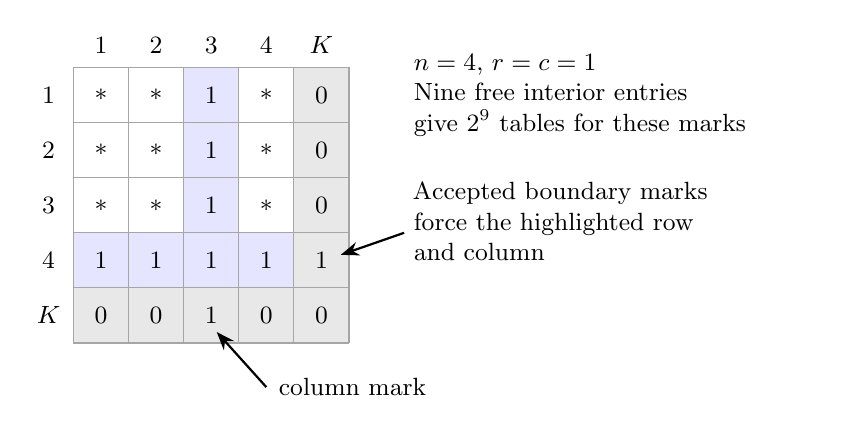
\begin{tikzpicture}[x=0.7cm,y=0.7cm,font=\small]
\fill[blue!10] (0,1) rectangle (4,2);
\fill[blue!10] (2,1) rectangle (3,5);
\fill[gray!18] (4,1) rectangle (5,5);
\fill[gray!18] (0,0) rectangle (5,1);
\draw[step=1,gray!70,thin] (0,0) grid (5,5);
\foreach \x in {0,1,2,3} {\node at (\x+.5,1.5) {$1$};}
\foreach \y in {2,3,4} {\node at (2.5,\y+.5) {$1$};}
\foreach \x in {0,1,3} {\foreach \y in {2,3,4} {\node at (\x+.5,\y+.5) {$*$};}}
\foreach \y in {2,3,4} {\node at (4.5,\y+.5) {$0$};}
\node at (4.5,1.5) {$1$};
\foreach \x in {0,1,3,4} {\node at (\x+.5,.5) {$0$};}
\node at (2.5,.5) {$1$};
\foreach \x/\lab in {0/1,1/2,2/3,3/4,4/K} {\node at (\x+.5,5.4) {$\lab$};}
\foreach \y/\lab in {4/1,3/2,2/3,1/4,0/K} {\node at (-.45,\y+.5) {$\lab$};}
\draw[-{Stealth},thick] (6.0,2.0) -- (4.85,1.6);
\node[anchor=west,align=left,text width=4.2cm] at (6,2.2)
 {Accepted boundary marks\\force the highlighted row\\and column};
\node[anchor=west,align=left,text width=5.0cm] at (6,4.5)
 {$n=4$, $r=c=1$\\Nine free interior entries\\give $2^9$ tables for these marks};
\draw[-{Stealth},thick] (3.5,-.8) -- (2.6,.2);
\node[anchor=west] at (3.55,-.8) {column mark};
\end{tikzpicture}
\caption{Boundary data, not accidental full interior rows, define the marks.
A $*$ is an arbitrary bit. The corner is rejected; accepting it gives the
single additional full table.}
\label{cta:fig:boundary}
\end{figure}

There are $\binom nr\binom nc$ choices of marks. Summing over $r,c$ and
adding the sole table with accepted corner proves the first identity
in \eqref{cta:eq:count}. To obtain the second, put $j=n-r$ and use
\[
 \sum_{c=0}^n\binom nc(2^j)^{n-c}=(1+2^j)^n.
\]
This also proves the formula at $n=0$: the double sum is $1$, and
$C_0=2$. The initial counts are
\begin{center}
\begin{tabular}{r r r}
\toprule
$n$ & $a_n$ & $C_n$\\
\midrule
0&1&2\\
1&5&6\\
2&47&48\\
3&1\,193&1\,194\\
4&113\,855&113\,856\\
5&46\,857\,665&46\,857\,666\\
6&83\,540\,629\,607&83\,540\,629\,608\\
\bottomrule
\end{tabular}
\end{center}
Different boundary patterns on an all-one interior are different tables.
They are correctly counted separately; only the full table with accepted
corner is supplied by the additional $1$.

\section{Bipartite graphs and the existing relational model}\label{cta:sec:graphs}

Take two distinguished labeled parts $L$ and $R$, each of size $n$.
A graph is any subset of $L\times R$, so there are $n^2$ independently
available edges. Write $i(G)$ for the total number of isolated vertices.

\begin{proposition}\label{cta:prop:graphs}
The sequence has the weighted graph interpretation
\begin{equation}\label{cta:eq:graphweight}
 a_n=\sum_G2^{i(G)}.
\end{equation}
For a uniform random graph in this model,
\begin{equation}\label{cta:eq:expectation}
 \frac{a_n}{2^{n^2}}=\E[2^{i(G)}],\qquad
 \E\binom{i(G)}k=P_k(n)2^{-nk}.
\end{equation}
\end{proposition}
\begin{proof}
Count pairs $(G,U)$ where $U$ is a subset of the isolated vertices.
Choose $r$ marked left vertices and $c$ marked right vertices. Their incident
edges must be absent and the other $(n-r)(n-c)$ edges are free, giving
exactly the double sum in \eqref{cta:eq:count}. For each fixed graph there are
$2^{i(G)}$ mark sets.

Directly, put an edge at each \emph{rejected} interior table entry. An
accepted boundary mark can only occur at an isolated vertex, and any
subset of isolated vertices can be marked. This is a bijection with the
closed tables having rejected corner.

For the second expectation, a specified collection of $r$ left and $k-r$
right vertices is isolated precisely when $nk-r(k-r)$ distinct edges
are absent. This event has probability $2^{-nk+r(k-r)}$. Sum over all
choices of the collection, using \eqref{cta:eq:P}. The first expectation
follows by dividing \eqref{cta:eq:graphweight} by $2^{n^2}$.
\end{proof}

Svato\v{s} et al. explicitly associate A196460 with the sentence
\begin{equation}\label{cta:eq:relational}
 (\forall x\,\forall y\ [U(x)\lor B(x,y)])\ \land\
 (\forall x\,\forall y\ [B(x,y)\lor U_1(y)])
\end{equation}
in Appendix A.1, Table 3, printed page 32 of version 1 \cite{svatos}.
The independent unary predicates $U,U_1$ choose active subsets of the
left and right copies of the domain. The relation $B$ must be true
except possibly at a pair whose two copies are active. Interpret a false
entry of $B$ as an edge. For any fixed graph, its nonisolated vertices
must be active, while each isolated vertex can be active or inactive,
yielding the weight $2^{i(G)}$ again. Although the relational structure
uses one domain, the graph uses two distinguished copies: $B(x,x)$
corresponds to an edge between copies, not a graph loop. All $n^2$ edge
choices remain available. This graph reading is a direct interpretation
of the existing sentence, not a claim to originate its combinatorial model.

\section{All fixed order forward asymptotics}\label{cta:sec:forward}

Dividing \eqref{cta:eq:count} by $2^{n^2}$ and grouping by $k=r+c$ gives the
exact finite identity
\begin{equation}\label{cta:eq:sectors}
 \As_n:=\frac{a_n}{2^{n^2}}
    =\sum_{k=0}^{2n}P_k(n)2^{-kn}.
\end{equation}
At a nonnegative integer $n$, $\binom nr=0$ for $r>n$, so the polynomial
formula \eqref{cta:eq:P} is valid even when $k>n$, and $P_k(n)=0$ for $k>2n$.
The same equality follows by averaging the finite identity
$2^{i(G)}=\sum_k\binom{i(G)}k$ in \eqref{cta:eq:expectation}.

Every $P_k$ has exact degree $k$ and positive leading coefficient
\begin{equation}\label{cta:eq:alpha}
 \alpha_k=\sum_{r=0}^k\frac{2^{r(k-r)}}{r!(k-r)!}.
\end{equation}
The first five polynomials are
\begin{align}\label{cta:eq:firstP}
 P_0(x)&=1,&P_1(x)&=2x,\notag\\
 P_2(x)&=3x^2-x,&
 P_3(x)&=\frac{13}{3}x^3-5x^2+\frac23x,\notag\\
 P_4(x)&=\frac{27}{4}x^4-\frac{33}{2}x^3+\frac{41}{4}x^2-\frac12x.
\end{align}
An exact finite regrouping alone is insufficient for an asymptotic
expansion: its number of terms grows with $n$. We next control that tail.

\begin{theorem}[Uniform tail for every fixed order]\label{cta:thm:tail}
For a fixed $M\geq0$ let
$R_{n,M}=\As_n-\sum_{k=0}^MP_k(n)2^{-kn}$.
If $n\geq M+1$ and $\rho_n:=2n2^{-n/2+1/4}<1$, then
\begin{equation}\label{cta:eq:explicit-tail}
 0\leq R_{n,M}\leq
 \frac{(2n)^{M+1}2^{-(M+1)n+(M+1)^2/4}}
      {(M+1)!(1-\rho_n)}
       +2^{2n-3n^2/4}.
\end{equation}
In particular \eqref{cta:eq:mainforward} holds. Its remainder is sharp:
\begin{equation}\label{cta:eq:forwardsharp}
 R_{n,M}\sim\alpha_{M+1}n^{M+1}2^{-(M+1)n}.
\end{equation}
\end{theorem}
\begin{proof}
Since $r(k-r)\leq k^2/4$, Vandermonde's identity gives, for $0\leq k\leq2n$,
\begin{equation}\label{cta:eq:majorant}
 0\leq P_k(n)2^{-kn}
 \leq B_{n,k}:=\binom{2n}k2^{-nk+k^2/4}.
\end{equation}
For $0\leq k<n$,
\[
 \frac{B_{n,k+1}}{B_{n,k}}
 =\frac{2n-k}{k+1}2^{-n+k/2+1/4}
 \leq2n2^{-n/2+1/4}=\rho_n.
\]
Consequently the sum over $M+1\leq k\leq n$ is at most
$B_{n,M+1}/(1-\rho_n)$. The inequality
$\binom{2n}{M+1}\leq(2n)^{M+1}/(M+1)!$ yields the first term of
\eqref{cta:eq:explicit-tail}.

On $[n,2n]$ the function $-nk+k^2/4$ is decreasing, with value
$-3n^2/4$ at $k=n$. Hence
\[
 \sum_{k=n+1}^{2n}B_{n,k}
 \leq2^{-3n^2/4}\sum_{k=n+1}^{2n}\binom{2n}k
 \leq2^{2n-3n^2/4}.
\]
This proves the explicit bound. Since $\rho_n\to0$, the first term is
$O_M(n^{M+1}2^{-(M+1)n})$. The second is little-oh of that scale:
the logarithm of their ratio has leading term $-3(\log2)n^2/4$.
This proves \eqref{cta:eq:mainforward}. For a concrete uniform range,
$n\geq\max(M+1,16)$ permits replacing $1/(1-\rho_n)$ by $2$:
$\rho_{16}<1/2$ and $\rho_n$ decreases thereafter.

Finally apply the already proved expansion with order $M+1$ and subtract
the truncation at $M$. Its first omitted term is
$P_{M+1}(n)2^{-(M+1)n}\sim\alpha_{M+1}n^{M+1}2^{-(M+1)n}$.
The next error divided by this scale is $O_M(n2^{-n})\to0$.
This proves \eqref{cta:eq:forwardsharp}.
\end{proof}

\wtag\ \emph{Relation to the transseries volume.} Theorem~\ref{cta:thm:tail}
is the A196460 analogue of Theorem~8.1 of \cite{cti}
(\texttt{t2:thm:graphs}), which proves every fixed exponential layer of
$c_n/2^{\binom n2}$ for connected labelled graphs with explicit polynomial
coefficients by the same device: a majorant whose successive ratios are
eventually below a constant less than one, plus a separate bound on the
quadratically small far range. That theorem is not cited by manuscript~21.

\wtag\ \emph{Second route to~\eqref{cta:eq:forwardsharp} (Part~II).}
Part~II's $R_{n,M}$ is the same tail. For $n\ge32$,
Theorem~\ref{cta:us:thm:sharp} gives
$R_{n,M}=P_{M+1}(n)2^{-(M+1)n}(1+E_{n,M})$ with $0\le E_{n,M}\le K_n=O(1/n)$,
uniformly in $0\le M<2n$; since $P_{M+1}$ has degree $M+1$ and leading
coefficient $\alpha_{M+1}$, this gives~\eqref{cta:eq:forwardsharp} again
for each fixed $M$, and Theorem~\ref{cta:us:thm:iff} extends the leading
equivalent to every order $M=M(n)$ with $M^2/n\to0$.

\begin{remark}[Fixed order does not mean convergence]\label{cta:rem:fixed}
The constants and the sufficiently large starting index may depend on $M$.
No estimate here is uniform for a truncation order growing with $n$.
For each integer $n$, \eqref{cta:eq:sectors} is finite; no claim is made that
$\sum_{k\geq0}P_k(x)2^{-kx}$ converges for noninteger $x$.
Formal power series used below require no such convergence.
\end{remark}

\subsection{The rarity of zero auxiliary arity}

The exact fraction of zero-auxiliary tables is
\begin{equation}\label{cta:eq:fraction}
 F_n=\frac{C_n}{2^{(n+1)^2}}
 =2^{-2n-1}\left(\As_n+2^{-n^2}\right).
\end{equation}
The additional full table contributes the isolated $2^{-n^2}$ inside
the parentheses. It is smaller than every fixed exponential sector as
$n\to\infty$. The first terms are therefore
\begin{equation}\label{cta:eq:rarity}
 F_n=2^{-2n-1}\left[1+2n2^{-n}+(3n^2-n)2^{-2n}
                    +O(n^3 2^{-3n})\right]
 \sim\frac12 4^{-n}=2^{1-2K}.
\end{equation}
The complementary fraction $1-F_n$ has exact minimum one positive
auxiliary by Theorem~\ref{cta:thm:classification}. At $n=0$ the exact formula
gives $F_0=1$, as both one-cell tables have minimum zero.

\section{Logarithmic coefficients and connected colored graphs}\label{cta:sec:logs}

In the formal ring $\mathbb Q[x][[z]]$ define $L_k$ by
\begin{equation}\label{cta:eq:logdef}
 \log\!\left(1+\sum_{k\geq1}P_k(x)z^k\right)
       =\sum_{k\geq1}L_k(x)z^k.
\end{equation}
Differentiating with respect to $z$ and multiplying by the series inside
the logarithm gives the explicit recurrence
\begin{equation}\label{cta:eq:Lrec}
 L_k=P_k-\frac1k\sum_{j=1}^{k-1}jL_jP_{k-j}\qquad(k\geq1).
\end{equation}
Induction shows $\deg L_k\leq k$. The first four are
\begin{align}\label{cta:eq:firstL}
 L_1(x)&=2x,\qquad L_2(x)=x^2-x,\notag\\
 L_3(x)&=x^3-3x^2+\frac23x,\notag\\
 L_4(x)&=\frac{19}{12}x^4-\frac{15}{2}x^3+\frac{101}{12}x^2-\frac12x.
\end{align}

\begin{proposition}[Actual logarithmic expansion]\label{cta:prop:log}
For every fixed $M\geq1$,
\begin{equation}\label{cta:eq:logasympt}
 \log_2 a_n=n^2+\frac1\la\sum_{k=1}^M L_k(n)2^{-kn}
            +O_M(n^{M+1}2^{-(M+1)n}),\qquad \la=\log2.
\end{equation}
\end{proposition}
\begin{proof}
Theorem~\ref{cta:thm:tail} at order zero gives
$u_n:=\As_n-1=O(n2^{-n})\to0$. For fixed $M$ it also gives
$u_n=\sum_{k=1}^MP_k(n)2^{-kn}+O_M(n^{M+1}2^{-(M+1)n})$.
The derivative of $\log(1+u)$ is bounded near $u=0$, so substituting this
truncation into the logarithm changes it by the same error order.
Its Taylor polynomial through power $M$ has remainder
$O(u_n^{M+1})=O_M(n^{M+1}2^{-(M+1)n})$.

Expand that finite Taylor polynomial. A term with total exponential index
$r$ has polynomial degree at most $r$. All retained terms of index
$r\leq M$ combine to $L_r(n)2^{-rn}$ by \eqref{cta:eq:logdef}.
There are only finitely many other terms, all with $r\geq M+1$;
they are bounded by $O_M(n^{M+1}2^{-(M+1)n})$ because $n2^{-n}\to0$.
Finally divide by $\la$ and add $n^2$.
\end{proof}

To understand the top coefficients, let $b_k=k!\alpha_k$, with $b_0=1$.
This counts simple graphs on $k$ labeled vertices equipped with a proper
coloring by two \emph{named} colors: choose the $r$ labels of the first
color and any of the $r(k-r)$ possible cross-color edges. These graphs
have a variable color split; they are not the balanced $n$-by-$n$ ambient
graphs counted in \eqref{cta:eq:graphweight}.

Let $c_k$ count the connected such colored graphs, where a singleton
has two color choices. A colored graph decomposes uniquely into its
connected colored components. Summing over partitions of its label set gives
\begin{equation}\label{cta:eq:expformula}
 \sum_{k\geq0}b_k\frac{z^k}{k!}
     =\exp\!\left(\sum_{k\geq1}c_k\frac{z^k}{k!}\right)
\end{equation}
formally. More explicitly, the coefficient at $z^k/k!$ on the right
sums $\prod_{B\in\pi}c_{|B|}$ over every set partition $\pi$ of the $k$
labels, which is exactly the component decomposition. Thus no analytic
convergence or random-graph connectivity theorem enters this identity.

Choosing the connected component containing label $1$ gives a constructive
recurrence:
\begin{equation}\label{cta:eq:crec}
 c_k=b_k-\sum_{j=1}^{k-1}\binom{k-1}{j-1}c_jb_{k-j}.
\end{equation}
Since $\deg P_k=k$, taking top-degree coefficients in \eqref{cta:eq:logdef}
amounts to taking the formal logarithm of $\sum\alpha_kz^k$.
Equation~\eqref{cta:eq:expformula} therefore proves
\begin{equation}\label{cta:eq:Lleading}
 [x^k]L_k(x)=\frac{c_k}{k!}>0.
\end{equation}
Positivity follows directly: the singleton works for $k=1$, and a
properly colored star supplies a connected example for every $k\geq2$.
For reference, the exact values retained by the independent audit are
\begin{center}
\begin{tabular}{r r r}
\toprule
$k$ & $b_k$ & $c_k$\\
\midrule
1&2&2\\2&6&2\\3&26&6\\4&162&38\\
5&1\,442&390\\6&18\,306&6\,062\\
7&330\,626&134\,526\\8&8\,488\,962&4\,172\,198\\
\bottomrule
\end{tabular}
\end{center}
\wtag\ These are OEIS A047863 ($b_k$, labelled graphs with two named proper
colours) and A002027 ($c_k$ for $k\ge1$; the entry's value at $k=0$ is $1$,
a separate convention) \cite{colored,connected}; manuscript~21 does not name
them, manuscript~24 does (Section~\ref{cta:us:sec:monomials}). The tabulated
values agree with both entries, and~\eqref{cta:eq:expformula} is the
relation between their exponential generating functions recorded in
A002027.

Applying Proposition~\ref{cta:prop:log} at one additional order also gives
the sharp logarithmic remainder
\begin{equation}\label{cta:eq:logsharp}
 \log_2a_n-n^2-\frac1\la\sum_{k=1}^M L_k(n)2^{-kn}
 \sim\frac{c_{M+1}}{\la(M+1)!}n^{M+1}2^{-(M+1)n}.
\end{equation}
In particular its sign is eventually positive for each fixed $M$.

\section{Formal inverse coefficients with an actual error proof}\label{cta:sec:inverse}

We first define a formal series; we then justify it on the actual
sequence values without introducing an interpolation of the sequence.
For coefficient extraction treat $s$ and $t$ as independent and work in
\[
 \mathbb Q[\la,\la^{-1},s,s^{-1}][[t]].
\]
Here $\la$ is a formal symbol in the algebra; subsequently it is evaluated
at $\log2>0$. Put $\delta_0=0$ and, recursively,
\begin{align}
 \delta_{m-1}(s,t)&=\sum_{j=1}^{m-1}D_j(s)t^j,\notag\\
 D_m(s)&=-\frac{1}{2s}[t^m]\left\{
 \delta_{m-1}(s,t)^2\right.\label{cta:eq:Drec}\\[-2pt]
 &\hspace{39mm}\left.{}+\frac1\la\sum_{k=1}^m
 L_k(s+\delta_{m-1}(s,t))t^k
 e^{-k\la\delta_{m-1}(s,t)}\right\}.\notag
\end{align}
Only finitely many Taylor coefficients contribute at each step. Equivalently,
$\delta=\sum_{j\geq1}D_j(s)t^j$ uniquely solves the formal equation
\begin{equation}\label{cta:eq:formal-inverse}
 2s\delta+\delta^2+
 \frac1\la\sum_{k\geq1}L_k(s+\delta)t^ke^{-k\la\delta}=0.
\end{equation}
At order $t^m$, the new $D_m$ occurs only in $2s\delta$. The square has
no constant term, and each summand already carries a positive power of $t$.
The coefficient of $D_m$ is therefore $2s$, invertible in this Laurent
ring, proving both the recurrence and uniqueness.

The first three coefficients are
\begin{align}\label{cta:eq:firstD}
 D_1(s)&=-\frac1\la,\notag\\
 D_2(s)&=-\frac{s+1}{2\la}+\frac{1}{2\la^2s},\notag\\
 D_3(s)&=-\frac{s^2}{2\la}-\frac{1}{3\la}
                      +\frac1{\la^2}+\frac1{\la^2s}.
\end{align}
The negative powers are harmless in the asymptotic region $s\to\infty$;
these formulas are not meant for evaluation at $s=0$.

\begin{lemma}[Degree bound and sign of the leading coefficient]\label{cta:lem:Ddegree}
The largest exponent of $s$ in $D_m$ is $m-1$, and
\begin{equation}\label{cta:eq:Dleading}
 D_m(s)\sim-\frac{c_m}{2\la m!}s^{m-1}.
\end{equation}
In particular $D_m(s)=O_m(s^{m-1})$ for $s\geq1$ as $s\to\infty$.
\end{lemma}
\begin{proof}
Induct on $m$. Assume every earlier $D_j$ has largest $s$ exponent at most
$j-1$. A product of $p$ earlier inverse coefficients with total $t$-degree
$m-k$ has largest $s$ exponent at most $m-k-p$. Derivatives of the polynomial
$L_k$ can only lower its degree from at most $k$; the exponential introduces
powers of $\la$ but no new powers of $s$. Thus every coefficient at
$t^m$ in the sum of \eqref{cta:eq:Drec} has exponent at most $m$ before division
by $s$. If any earlier $D_j$ occurs, then $p\geq1$ and the bound is
strictly less than $m$. The term $\delta_{m-1}^2$ has exponent at most
$m-2$. The only possible contribution at exponent $m$ is therefore
$\la^{-1}L_m(s)$, whose coefficient is $c_m/(\la m!)$ by
\eqref{cta:eq:Lleading}. Division by $-2s$ proves both the exact top degree
and \eqref{cta:eq:Dleading}. This also covers $m=1$.
\end{proof}

\begin{theorem}[Sequence-point inversion and its sharp sign]\label{cta:thm:inverse}
For $s_n=\sqrt{\log_2a_n}$, $t_n=2^{-s_n}$ and each fixed $M\geq1$,
\begin{equation}\label{cta:eq:inversebound}
 n-\left(s_n+\sum_{k=1}^MD_k(s_n)t_n^k\right)
       =O_M(s_n^M t_n^{M+1}).
\end{equation}
More sharply,
\begin{equation}\label{cta:eq:inversesharp}
 n-\left(s_n+\sum_{k=1}^MD_k(s_n)t_n^k\right)
 \sim-\frac{c_{M+1}}{2\la(M+1)!}s_n^M t_n^{M+1}.
\end{equation}
Every fixed truncation consequently overestimates the integer $n$
for all sufficiently large $n$.
\end{theorem}
\begin{proof}
Fix $M$ and introduce the \emph{finite} smooth function
\begin{equation}\label{cta:eq:proxy}
 H_M(x)=x^2+\frac1\la\sum_{k=1}^ML_k(x)2^{-kx}.
\end{equation}
This is an explicit approximation, not an interpolation of $a_n$.
Proposition~\ref{cta:prop:log} gives at the actual integer $n$
\begin{equation}\label{cta:eq:resid1}
 H_M(n)-s_n^2=O_M(n^{M+1}2^{-(M+1)n}).
\end{equation}
It also gives $s_n^2-n^2=O(n2^{-n})$. Division by $s_n+n$, which is
at least $2n$ because $a_n\geq2^{n^2}$, yields
\begin{equation}\label{cta:eq:closeness}
 s_n-n=O(2^{-n}),\qquad n\sim s_n,\qquad 2^{-n}/t_n\longrightarrow1.
\end{equation}
Define $\widehat n_M=s_n+\delta_M(s_n,t_n)$, where
$\delta_M(s,t)=\sum_{j=1}^MD_j(s)t^j$.
Lemma~\ref{cta:lem:Ddegree} and $st\to0$ imply $\delta_M(s,t)=O_M(t)$
along $t=2^{-s}$. Hence both $n$ and $\widehat n_M$ lie in
$[s_n-1,s_n+1]$ for all sufficiently large $n$.

We detail the residual bound at $\widehat n_M$, since purely formal
cancellation is not an analytic error estimate. Substitute $s+\delta_M$
into \eqref{cta:eq:proxy}, set $t=2^{-s}$, and subtract $s^2$:
\begin{equation}\label{cta:eq:residualformula}
 2s\delta_M+\delta_M^2+
 \frac1\la\sum_{k=1}^ML_k(s+\delta_M)t^ke^{-k\la\delta_M}.
\end{equation}
Expand the finite polynomials exactly. In the term with prefactor $t^k$,
expand the exponential through power $M-k$ of $\delta_M$. The exponential
remainder is $O_M(\delta_M^{M-k+1})$, uniformly for small $\delta_M$.
As $L_k(s+\delta_M)=O_M(s^k)$ and $\delta_M=O_M(t)$, its contribution
is $O_M(s^kt^{M+1})$, hence $O_M(s^{M+1}t^{M+1})$.

The remaining expression is a finite polynomial in $t$ with Laurent
coefficients in $s$. All coefficients through order $M$ vanish by
\eqref{cta:eq:Drec}. Every remaining coefficient of $t$-degree $r$ has
largest $s$ exponent at most $r$: for $2s\delta_M$ this follows from
Lemma~\ref{cta:lem:Ddegree}; for $\delta_M^2$ the stronger bound $r-2$ holds;
and for each expanded logarithmic summand the same product-degree
argument as in that lemma gives at most $r$.
Thus each of its finitely many terms with $r\geq M+1$ is
$O_M(s^rt^r)=O_M(s^{M+1}t^{M+1})$, since $s\geq1$ and $st\to0$.
Negative powers only improve this bound. We have proved
\begin{equation}\label{cta:eq:resid2}
 H_M(\widehat n_M)-s_n^2
       =O_M(s_n^{M+1}t_n^{M+1}).
\end{equation}

Differentiating only the finite function \eqref{cta:eq:proxy}, uniformly on
$[s_n-1,s_n+1]$, gives
\[
 H_M'(x)=2x+O_M(x^M2^{-x})\geq s_n
\]
for large $n$. Subtract \eqref{cta:eq:resid1} from \eqref{cta:eq:resid2}, use
\eqref{cta:eq:closeness} to compare the error scales, and apply the mean-value
theorem between $n$ and $\widehat n_M$. Dividing by the derivative lower
bound $s_n$ proves \eqref{cta:eq:inversebound}.

Finally use the proved bound at order $M+1$. The difference at order $M$
is $D_{M+1}(s_n)t_n^{M+1}+O_M(s_n^{M+1}t_n^{M+2})$. The ratio of the
last error to $s_n^Mt_n^{M+1}$ tends to zero because $s_nt_n\to0$.
Lemma~\ref{cta:lem:Ddegree} proves \eqref{cta:eq:inversesharp} and its negative sign.
\end{proof}

\wtag\ \emph{Relation to the transseries volume.} The proof is the method
of Corollary~8.2 of \cite{cti} (\texttt{t2:cor:graph-range}): a finite
smooth forward model, the residual of the formal inverse at the sequence
value, and division by a lower bound for the slope, which is the local
inverse certificate of its Theorem~2.12 (\texttt{t1:thm:certificate}); in
both, the quadratic core needs no Lambert function and no interpolation of
the sequence is used. Here the core is $x^2$ in the coordinate
$s=\sqrt{\log_2a_n}$, there $\tfrac{\log2}2x(x-1)$. The sharp signed
remainder~\eqref{cta:eq:inversesharp} has no counterpart there.

\subsection{Replacing the sequence by the table count}

Since $C_n=a_n+1$ and $a_n\geq2^{n^2}$,
\begin{equation}\label{cta:eq:Cchange}
 \log_2C_n-\log_2a_n=\log_2(1+a_n^{-1})=O(2^{-n^2}).
\end{equation}
For $n\to\infty$, the square-root difference is $O(2^{-n^2}/n)$.
Both are smaller than every fixed error sector above. Thus all fixed-order
forward, logarithmic and inverse expansions, including their sharp
remainder equivalents, hold with $C_n$ in place of $a_n$ and
$s_n=\sqrt{\log_2C_n}$. This is an asymptotic statement; it does not erase
the different exact endpoint at $n=0$.

\section{Exact integer thresholds and the floor boundary}\label{cta:sec:threshold}

The double sum immediately gives, for every $n\geq0$,
\begin{equation}\label{cta:eq:brackets}
 2^{n^2}\leq a_n\leq2^{n^2+2n}<2^{(n+1)^2}.
\end{equation}
The lower bound is the term $r=c=0$. For the upper bound replace each
$2^{(n-r)(n-c)}$ by $2^{n^2}$ and sum the binomial weights to obtain $4^n$.
Consequently
\begin{equation}\label{cta:eq:floorpoint}
 \left\lfloor\sqrt{\log_2a_n}\right\rfloor=n
 \quad\text{for every }n\geq0,
\end{equation}
including $a_0=1$. Also $a_n$ is strictly increasing: each old $j\leq n$
term of the single sum for $a_{n+1}$ is at least twice the corresponding
term for $a_n$, because $\binom{n+1}{j}\geq\binom nj$ and $1+2^j\geq2$;
there is an additional positive term at $j=n+1$.

\begin{theorem}[One exact comparison suffices]\label{cta:thm:threshold}
For real $y\geq1$ put $m=\lfloor\sqrt{\log_2y}\rfloor$. Then
\begin{equation}\label{cta:eq:exactinverse}
 N_a(y):=\max\{n\geq0:a_n\leq y\}
   =\begin{cases}m-1,&y<a_m,\\m,&y\geq a_m.\end{cases}
\end{equation}
At $m=0$ only the second branch occurs. Below $y=1$ the defining set is empty.
For $C_n$, the same two-branch rule with $C_m$ in place of $a_m$ holds
for all $y\geq2$; below $2$ its defining set is empty.
\end{theorem}
\begin{proof}
If $n<m$, then \eqref{cta:eq:brackets} gives
$a_n<2^{(n+1)^2}\leq2^{m^2}\leq y$. If $n>m$, then
$a_n\geq2^{n^2}\geq2^{(m+1)^2}>y$. Only index $m$ remains undecided,
and its exact comparison yields \eqref{cta:eq:exactinverse}.
When $m=0$, $y\geq1=a_0$, so the first branch cannot arise.

For $n\geq1$, adding one to \eqref{cta:eq:brackets} still gives
$2^{n^2}<C_n<2^{(n+1)^2}$, since
$2^{n^2+2n}+1<2^{n^2+2n+1}$. But $C_0=2$ equals $2^{1^2}$.
If $y\geq2$, then $m\geq1$. We have $C_{m-1}\leq2^{m^2}\leq y$,
with equality in the first inequality possible at $m=1$; all indices
above $m$ fail. Strict increase of $C_n$ and comparison with $C_m$
prove the claim.
\end{proof}

The sequence-point floor \eqref{cta:eq:floorpoint} holds for $C_n$ when
$n\geq1$, but \emph{fails at zero}:
$\lfloor\sqrt{\log_2C_0}\rfloor=1$. In contrast the threshold theorem
correctly gives $N_C(2)=0$.

\wtag\ \emph{Relation to the staircase theorem.} $N_a(y)=\max\{n:a_n\le y\}$
is the floor-type companion of the integer staircase
$N_\ast(y)=\min\{n:a_n\ge y\}$ of the canonical volume \cite[Theorem~J.43,
\texttt{p0:thm:staircase}]{tsvol}: the two agree at the sequence values and
$N_a=N_\ast-1$ strictly between them. That theorem obtains $N_\ast$ by
rounding an admissible interpolation's inverse, or by a separation
condition on an approximate inverse; Theorem~\ref{cta:thm:threshold}
needs neither, because the brackets~\eqref{cta:eq:brackets} leave a single
candidate index and one exact comparison, the route that Chapter~8 of
\cite{cti} names (``bracketing consecutive exact counts''). The paragraph
after Figure~\ref{cta:fig:threshold} is the separation condition in this
setting.

To locate the threshold in logarithmic coordinates, expand the square
root in Proposition~\ref{cta:prop:log}. With $q=2^{-m}$,
\begin{equation}\label{cta:eq:boundaryshift}
 \sqrt{\log_2a_m}
 =m+\frac q\la+
 \left(\frac{m-1}{2\la}-\frac{1}{2\la^2m}\right)q^2
 +O(m^2q^3).
\end{equation}
Indeed, $L_1(m)=2m$ contributes $q/\la$; $L_2(m)=m^2-m$
contributes $(m-1)q^2/(2\la)$; and the quadratic square-root term
contributes $-q^2/(2\la^2m)$. The next logarithmic term and all remaining
square-root terms are $O(m^2q^3)$. This is an expansion for $m\to\infty$,
not a formula to be evaluated at $m=0$.

\begin{figure}[htbp]
\centering
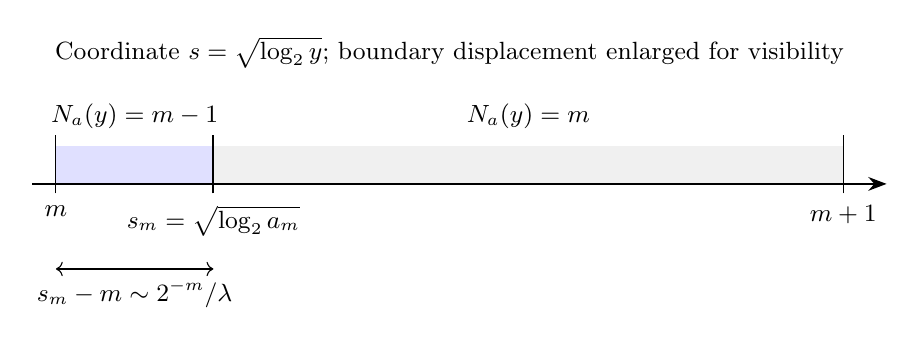
\begin{tikzpicture}[x=1cm,y=1cm,font=\small]
\fill[blue!12] (0,0) rectangle (2,0.48);
\fill[gray!12] (2,0) rectangle (10,0.48);
\draw[-{Stealth},thick] (-.3,0) -- (10.55,0);
\draw (0,-.12)--(0,.62);
\draw[thick] (2,-.12)--(2,.62);
\draw (10,-.12)--(10,.62);
\node[below] at (0,-.15) {$m$};
\node[below,align=center] at (2,-.15) {$s_m=\sqrt{\log_2a_m}$};
\node[below] at (10,-.15) {$m+1$};
\node at (1,.86) {$N_a(y)=m-1$};
\node at (6,.86) {$N_a(y)=m$};
\node[above,align=center] at (5,1.35)
 {Coordinate $s=\sqrt{\log_2y}$; boundary displacement enlarged for visibility};
\draw[<->] (0,-1.08)--(2,-1.08);
\node[below] at (1,-1.1) {$s_m-m\sim2^{-m}/\la$};
\end{tikzpicture}
\caption{Within $m\leq\sqrt{\log_2y}<m+1$, the exact threshold is $a_m$.
The boundary itself belongs to the right-hand interval. The diagram is
schematic: the left interval has exponentially small width.}
\label{cta:fig:threshold}
\end{figure}

Thus $N_a(y)$ differs from $m$ precisely when
$m\leq\sqrt{\log_2y}<\sqrt{\log_2a_m}$. An approximate boundary may classify
$y$ only when its distance from the true comparison boundary exceeds a
\emph{proved} error bound. Inside an uncertainty interval, use the exact
comparison in \eqref{cta:eq:exactinverse}. Neither a bare big-oh statement nor
flooring a truncated real inverse automatically produces an exact integer
answer. Formula~\eqref{cta:eq:boundaryshift} has the same fixed-order expansion
for $C_m$, with only the beyond-all-fixed-orders perturbation
\eqref{cta:eq:Cchange}.

\section{Exact numerical evidence and its logical role}\label{cta:sec:evidence}

The source packet contains exact arithmetic checks through order six;
a separate fresh independent audit extends formal checking through order
eight \cite{source,audit}. The independently authored algebra checker
derives inverse coefficients using the \emph{exponentiated} equation
\begin{equation}\label{cta:eq:alternative}
 \sum_{k\geq0}P_k(s+\delta)t^k
 \exp\!\bigl(\la((2s-k)\delta+\delta^2)\bigr)=1,
\end{equation}
whose new linear coefficient is $2\la s$, and checks cancellation in both
this equation and \eqref{cta:eq:formal-inverse}. This is a useful independent
algebraic route, though finite-order cancellation cannot establish the
infinite family of estimates proved above.

The retained independent results include:
\begin{itemize}
\item all $66\,066$ Boolean tables for $K=1,2,3,4$, with closed counts
$2,6,48,1194$, and $44\,298$ direct zero-polynomial evaluations;
\item all $66\,067$ bipartite graphs for $n=0,1,2,3,4$, checking their
weighted sums and every isolation factorial moment;
\item $33\,868$ ordinary labeled graphs on $0$ through $6$ vertices,
checking the colored counts by bipartiteness and connected components;
\item $65$ sequence indices $n=0,\ldots,64$, $585$ values of the
coefficient polynomials, and $4\,225$ exact majorant comparisons;
\item $1\,012$ rational inverse-threshold comparisons, including small
endpoints and probes on both sides of sequence and square boundaries;
\item inverse cancellation through order eight, all displayed
coefficients, the three leading-coefficient identities, and agreement
with all $21$ source coefficient families through order six.
\end{itemize}
The majorants are checked after fourth powers so that no floating fourth
root is required. Threshold floors are checked using integer bit lengths,
integer square roots, and exact rational comparison, avoiding accidental
rounding at boundaries.
\wtag\ The list above is the independent audit's (shipped as
\path{code/21-fixed-audit-check_mathematics.py} with its record
\path{data/21-fixed-audit-ev-mathematics.json}). The source packet's own
checker (\path{code/21-fixed-src-verify_exact.py},
\path{data/21-fixed-src-ev-exact.json}) covers the same $66\,066$ tables and
$66\,067$ graphs, $33$ sequence indices $n=0,\ldots,32$, $231$ polynomial
values and formal inverse cancellation through order six; its companion
\path{code/21-fixed-src-verify_connected.py} checks the three
leading-coefficient identities through order six.

A separate retained interval check encloses $s_n$, $t_n$ and the signed
inverse error using rational arithmetic: a positive atanh series with a
geometric tail for logarithms, integer square roots for square roots,
alternating Taylor bounds for $e^{-x}$, and outward $1024$-bit dyadic
rounding after arithmetic. All $36$ cases with $n=16,32,64$, orders
$M=1,\ldots,6$, and sequences $a,C$ have a strictly negative upper
endpoint for the inverse remainder.

For the $a$ sequence, write
\[
 \Rinv_{n,M}=n-s_n-\sum_{k=1}^MD_k(s_n)t_n^k,\qquad
 J_{n,M}=-\frac{c_{M+1}}{2\la(M+1)!}s_n^Mt_n^{M+1}.
\]
Table~\ref{cta:tab:ratios} reproduces selected decimal \emph{outward enclosures}
from the retained exact endpoints. The ratio tends to one for each fixed
$M$ by Theorem~\ref{cta:thm:inverse}; the table illustrates both approach
directions and the slower onset at a larger truncation order.

\begin{table}[htbp]
\centering
\small
\begin{tabular}{r r l}
\toprule
$n$ & $M$ & Enclosure for $\Rinv_{n,M}/J_{n,M}$\\
\midrule
16&1&$[1.057106335697,\ 1.057106335698]$\\
32&1&$[1.029841125557,\ 1.029841125558]$\\
64&1&$[1.015272779531,\ 1.015272779532]$\\[2pt]
16&3&$[0.893719133773,\ 0.893719133774]$\\
32&3&$[0.948737227650,\ 0.948737227651]$\\
64&3&$[0.974858114102,\ 0.974858114103]$\\[2pt]
16&6&$[0.532599538158,\ 0.532599538159]$\\
32&6&$[0.741284482732,\ 0.741284482733]$\\
64&6&$[0.864003938458,\ 0.864003938459]$\\
\bottomrule
\end{tabular}
\caption{Selected rigorous inverse-error ratios from the independent audit.
These are retained numerical evidence, not newly rerun computations for
this article and not a substitute for the fixed-order proof.}
\label{cta:tab:ratios}
\end{table}

\section{Further questions and the limits of the results}\label{cta:sec:questions}

\paragraph{Growing truncation order.}
The proof fixes $M$ before letting $n$ grow. What is the widest useful
range $M=M(n)$ for which a comparably precise remainder can be established?
The factor $2^{r(k-r)}$ in \eqref{cta:eq:P} grows rapidly with the sector index,
so degree estimates alone do not settle this question. A useful answer
would have to control the transition between the small-$k$ regime and the
large-$k$ tail, rather than assert convergence of the fixed-order expansion.

\wtag\ \emph{Answered in part by Part~II.} For the exact sector tail, Part~II
answers this question with all orders at once: for $n\ge32$ and every
$0\le M<2n$ the tail exceeds its first omitted sector by a relative amount
at most $K_n\sim9/(13n)$, attained only at $M=2n-4$
(Theorem~\ref{cta:us:thm:sharp}), and by at most $1/n$ for $C_n$ with the
extra table merged into the terminal sector
(Theorem~\ref{cta:us:thm:merged}). Replacing the coefficient $P_k(n)$ by its
leading monomial is accurate exactly when $k^2/n\to0$
(Theorem~\ref{cta:us:thm:iff}), and with an explicit correction for
$k=o(n^{2/3})$ (Theorem~\ref{cta:us:thm:corrected}). The question remains
open for the logarithmic and inverse expansions of
Sections~\ref{cta:sec:logs} and~\ref{cta:sec:inverse}
(Section~\ref{cta:us:sec:scope}).

\paragraph{Rectangular and higher dimensional tables.}
For a table with $p$ finite row labels and $q$ finite column labels, the
same boundary argument immediately gives
\[
 C_{p,q}=1+\sum_{r=0}^p\sum_{c=0}^q
           \binom pr\binom qc2^{(p-r)(q-c)}.
\]
This is a direct counting consequence, but asymptotics when $p/q$ varies
or one side stays bounded require their own error analysis. In dimension
at least three the coordinate-flat criterion and one-positive-witness
formula extend, while boundary faces overlap in a more complicated pattern.
A useful next problem is an exact counting representation that organizes
those overlaps without double counting.

\wtag\ The extension to dimension $d\ge3$ is Report~69's ``fixed-dimensional
extension'' \cite{smc}, which states the classification for every fixed
finite dimension with the same single-equation, positive-integer and
unrestricted-degree qualifications.

\paragraph{Effective inverse certification.}
The finite proxy proof yields an error order and the exact threshold
rule yields a final integer answer. Can explicit derivative and Taylor
constants be combined into a practical certified interval procedure that
usually avoids forming the full integer $a_m$? The goal would be a
proved stopping criterion, with exact comparison when the interval
straddles the threshold. The asymptotic expansion by itself provides no
such universal rounding guarantee.

\paragraph{Representation cost inside the zero-auxiliary class.}
The polynomial \eqref{cta:eq:zeropoly} gives degree $2|S|$ when $S$ is nonempty
and has no all-tail cell. It need not minimize degree, coefficient height,
or number of monomials. Characterizing these costs within the closed tables
is separate from minimizing auxiliary arity. The present count does not
answer that optimization problem.

\paragraph{Scope.}
All proofs concern fixed finite tables on positive integer inputs and one
polynomial equality. All asymptotic expansions are at fixed order. Formal
series manipulations are justified only by the finite truncations and
error arguments given here. In particular the ordinary and exponential
generating functions of $a_n$ both have analytic radius zero, since
$a_n\geq2^{n^2}$ implies both $a_n^{1/n}\to\infty$ and
$(a_n/n!)^{1/n}\to\infty$. They can still be interpreted formally.
No physical simulation, source interpreter, saved schedule or theorem
prover was run to prepare this article. No external submission or novelty
claim is implied by its preparation.

\part{Sharp uniform finite sector truncations of A196460}\label{cta:us:part}

\wtag\ Part~II is manuscript~24 of batch~91, the article \emph{Sharp
uniform finite sector truncations of A196460}, author line ``A companion
mathematical article'', dated 4 October 2026 (12 pages as delivered). Its
title block is replaced by this Part heading; its abstract and keywords
follow unchanged, and its text has the label prefix \texttt{cta:us:} and
the \wtag\ notes. Its ``companion article'' \cite{fixed} is Part~I.

\begin{quotation}
\small
\noindent\textbf{Abstract of Part~II.}
The normalized terms of OEIS A196460 have an exact decomposition into
$2n+1$ positive sectors. For every $n\ge32$, we determine the largest
relative excess of a tail over its first omitted sector, simultaneously
over every truncation order $0\le M<2n$. The unique worst truncation is
$M=2n-4$, its excess is an explicit rational function, and the optimal
asymptotic uniform constant is $9/13$. For the clipping-table count
$C_n=1+a_n$, merging the extra contribution into the terminal sector
changes the exact maximum to $1/n$, attained uniquely at $M=2n-2$.
Complement symmetry, a raising identity, and estimates on both
discrete-Gaussian lattices give elementary proofs. Separately, a sector
coefficient is asymptotic to its leading monomial precisely when
$k^2/n\to0$; an explicit central correction remains uniform for
$k=o(n^{2/3})$ and yields the transition $e^{-c^2/4}$ at
$k\sim c\sqrt n$. The finite-sector conclusions neither provide a
growing-order inverse expansion nor justify replacing all earlier
coefficients by their leading terms. The threshold $32$ is convenient,
not asserted minimal. No novelty or priority claim is made.

\smallskip
\noindent\textbf{Keywords.} A196460; finite sector expansions; sharp uniform
tails; discrete Gaussian; clipping tables; growing-order asymptotics.

\end{quotation}

\section{The exact sectors and the scope of the question}\label{cta:us:sec:setup}

For an integer $n\ge1$, let
\begin{equation}\label{cta:us:eq:an}
 a_n=\sum_{j=0}^n\binom nj(1+2^j)^n.
\end{equation}
This is OEIS A196460, entered by Paul D. Hanna in 2011; the leading
asymptotic $a_n\sim2^{n^2}$ is credited there to V\'aclav Kotesovec in
2013 \cite{oeis}. Define, for $0\le k\le2n$,
\begin{equation}\label{cta:us:eq:sectors}
 P_k(n)=\sum_{\substack{r+c=k\\0\le r,c\le n}}
       \binom nr\binom nc2^{rc},\qquad
 S(n,k)=P_k(n)2^{-nk},\qquad A_n=\frac{a_n}{2^{n^2}}.
\end{equation}
Each $P_k(n)$ is strictly positive: every allowed $k$ admits at least
one pair $(r,c)$ in the indicated square. Expanding \eqref{cta:us:eq:an},
then replacing both binomial indices by their complements, gives
\begin{align}\label{cta:us:eq:normalization}
 a_n&=\sum_{u,v=0}^n\binom nu\binom nv2^{uv}
     =\sum_{r,c=0}^n\binom nr\binom nc2^{(n-r)(n-c)},\notag\\
 A_n&=\sum_{r,c=0}^n\binom nr\binom nc2^{-n(r+c)+rc}
     =\sum_{k=0}^{2n}S(n,k).
\end{align}
Thus the sector decomposition is finite and exact, including both endpoints.

\wtag\ This is Part~I's identity~\eqref{cta:eq:sectors}, re-derived; $A_n$
is Part~I's $\As_n$, and $P_k(n)$ is Part~I's polynomial~\eqref{cta:eq:P} at
the integer $n$.

The companion article \cite{fixed} proves the zero-auxiliary-variable
classification for Boolean tables clipped at $K=n+1$, as well as the count
$C_n=1+a_n$. Briefly, an accepted boundary mark forces its full row or
column; with the tail corner rejected, $r$ row marks and $c$ column marks
leave $(n-r)(n-c)$ free interior entries. Summing their choices gives the
double sum in \eqref{cta:us:eq:normalization}. The accepted corner forces the
single full table, accounting for the extra $1$. We use this established
count without repeating its closure classification or inverse theory.

\wtag\ The companion is Part~I of this report: the classification is
Section~\ref{cta:sec:closure} (Report~69's theorem, \cite{smc}), the count
Section~\ref{cta:sec:count}, the graph interpretation
Section~\ref{cta:sec:graphs}, and the inverse theory
Sections~\ref{cta:sec:logs}--\ref{cta:sec:threshold}.

The same companion explains the graph interpretation
$a_n=\sum_G2^{i(G)}$: $G$ ranges over graphs on two distinguished labeled
parts of size $n$, and $i(G)$ counts isolated vertices. Choosing a subset
of isolated vertices marks the boundary. Its sector interpretation is
$S(n,k)=\E\binom{i(G)}k$ for the uniform random graph. This is consistent
with the existing two-unary, one-binary relational model for A196460 in
Svato\v{s} et al.\ \cite{svatos}; the two graph parts are distinct copies
of the domain, so all $n^2$ edges, including pairs of corresponding labels,
remain available. These interpretations are credited background, not
claims of a new model.

For every allowed truncation order, put
\begin{equation}\label{cta:us:eq:excess}
 R_{n,M}=\sum_{k=M+1}^{2n}S(n,k),\qquad
 E_{n,M}=\frac{R_{n,M}}{S(n,M+1)}-1,
 \qquad 0\le M<2n.
\end{equation}
The question here is stronger than a statement for each fixed $M$:
how well does the first omitted \emph{exact} sector approximate the tail,
uniformly over all $2n$ possible values of $M$?

\begin{theorem}[Exact sharp bound for every truncation]\label{cta:us:thm:sharp}
For every integer $n\ge32$, simultaneously for all integers $0\le M<2n$,
\begin{equation}\label{cta:us:eq:sharp}
 0\le E_{n,M}\le K_n,
 \qquad K_n=\frac{3(3n^2+n+1)}{n(13n^2-15n+2)}.
\end{equation}
The upper equality holds uniquely at $M=2n-4$. Moreover,
\begin{equation}\label{cta:us:eq:Kcorrection}
 K_n=\frac{9}{13n}
     +\frac{174n+21}{13n(13n^2-15n+2)},\qquad
 \lim_{n\to\infty}\max_{0\le M<2n}nE_{n,M}=\frac9{13}.
\end{equation}
In particular $9/13$ is the optimal asymptotic uniform constant.
\end{theorem}

\begin{theorem}[Sharp bound for the clipping-table count]\label{cta:us:thm:merged}
Let $C_n=a_n+1$, and merge its additional normalized contribution into
the terminal sector only:
\begin{equation}\label{cta:us:eq:merged}
 S_C(n,k)=
 \begin{cases}S(n,k),&0\le k<2n,\\2S(n,2n),&k=2n.
 \end{cases}
 \qquad \frac{C_n}{2^{n^2}}=\sum_{k=0}^{2n}S_C(n,k).
\end{equation}
For $n\ge32$, simultaneously for $0\le M<2n$,
\begin{equation}\label{cta:us:eq:Csharp}
 0\le E^C_{n,M}:=
 \frac{\sum_{k=M+1}^{2n}S_C(n,k)}{S_C(n,M+1)}-1\le\frac1n.
\end{equation}
The upper equality holds uniquely at $M=2n-2$. At $M=2n-1$ the
relative excess is zero. The sharp asymptotic uniform constant in this
merged convention is therefore $1$.
\end{theorem}

The threshold $32$ in both statements is chosen for the elementary
estimates below. No minimal-threshold assertion is intended. Also,
the normalization in Theorem~\ref{cta:us:thm:merged} matters: if the additional
$2^{-n^2}$ is left outside the sectors and the old denominator $S$ is
used, the excess at $M=2n-1$ is exactly $1$, not $O(1/n)$.

\section{Complement symmetry and the raising identity}\label{cta:us:sec:identities}

Two exact identities connect the middle of the sector range with its
ends. First, substituting $r=n-u$, $c=n-v$ gives
\[
 -n(r+c)+rc=-n^2+uv.
\]
Binomial symmetry therefore proves
\begin{equation}\label{cta:us:eq:complement}
 S(n,2n-k)=2^{-n^2}P_k(n),\qquad 0\le k\le2n.
\end{equation}
In particular $P_0(n)=1$ and $S(n,2n)=2^{-n^2}$, which explains
the terminal merge in \eqref{cta:us:eq:merged}.

Write $w_{r,c}=\binom nr\binom nc2^{rc}$, with all sums below restricted
to valid $r,c$. For $0\le k<2n$, the raising identity is
\begin{equation}\label{cta:us:eq:raising}
 (k+1)P_{k+1}(n)=\sum_{r+c=k}w_{r,c}
                   \bigl[(n-r)2^c+(n-c)2^r\bigr].
\end{equation}
Indeed, $(n-r)\binom nr=(r+1)\binom n{r+1}$, and multiplication by
$2^c$ changes $2^{rc}$ to $2^{(r+1)c}$. Raising the first coordinate
therefore gives a target weight times its new first coordinate; raising
the second gives that weight times its new second coordinate. Every
target of total degree $k+1$ is counted with total multiplier $k+1$.
Forbidden boundary moves have factor $n-r=0$ or $n-c=0$. This argument
also covers $k=0$ and $k=2n-1$.

Set
\[
 \la=\log2,\qquad h=r-k/2,\qquad D=n-k/2.
\]
The bracket in \eqref{cta:us:eq:raising} equals
\begin{equation}\label{cta:us:eq:hyperbolic}
 2^{k/2}\bigl[2D\cosh(\la h)+2h\sinh(\la h)\bigr].
\end{equation}
Here $D>0$ for $k<2n$, $\cosh(\la h)\ge1$, and
$h\sinh(\la h)\ge0$. Dividing the sum by the positive $P_k(n)$ proves
\begin{equation}\label{cta:us:eq:raise-lower}
 \frac{P_{k+1}(n)}{P_k(n)}\ge
 \frac{2n-k}{k+1}2^{k/2},\qquad 0\le k<2n.
\end{equation}

For a high-sector ratio, put $\ell=2n-k$. If $n\le k<2n$, then
$1\le\ell\le n$; complement symmetry and \eqref{cta:us:eq:raise-lower} at
$\ell-1$ give
\begin{equation}\label{cta:us:eq:g}
 \frac{S(n,k+1)}{S(n,k)}
 =\frac{P_{\ell-1}(n)}{P_\ell(n)}
 \le g_{n,\ell}:=
 \frac{\ell\,2^{-(\ell-1)/2}}{2n-\ell+1}
 \le q_n:=\frac{3}{2(n+1)}.
\end{equation}
For the last inequality, the numerator has values $1,\sqrt2,3/2$ at
$\ell=1,2,3$, and thereafter its next-to-current ratio is
$(\ell+1)/(\sqrt2\ell)<1$. Its exact maximum is thus $3/2$.
The denominator is at least $n+1$ throughout $1\le\ell\le n$.

\section{Both discrete Gaussian lattices and every adjacent ratio}\label{cta:us:sec:gaussian}

To control low sectors we need an upper, rather than a lower, bound in
\eqref{cta:us:eq:raising}. At fixed $k$, its normalized summand weights in $h$
are proportional to
\begin{equation}\label{cta:us:eq:weighted-gaussian}
 b(h)2^{-h^2},\qquad
 b(h)=\binom n{k/2+h}\binom n{k/2-h}.
\end{equation}
The lattice is $\Z$ for even $k$ and $\Z+\tfrac12$ for odd $k$.
The factor $2^{k^2/4}$ cancels on normalizing. Extend $b$ by zero outside
the allowed finite support. It is symmetric, and for nonnegative $h$
where the ratio is defined,
\begin{equation}\label{cta:us:eq:bmono}
 \frac{b(h+1)}{b(h)}
 =\frac{(D-h)(k/2-h)}{(k/2+h+1)(D+h+1)}\le1.
\end{equation}
At the edge of the support the next value is zero, and beyond that
$b$ remains zero. Thus $b$ decreases with $|h|$, including the
degenerate supports at $k=0,1$.

\begin{lemma}[Decreasing reweighting]\label{cta:us:lem:reweight}
On either of the two lattices, give $h$ probability proportional to
$2^{-h^2}$. If $b$ is nonnegative, symmetric, decreasing with $|h|$,
and has positive mean, then for every integrable nonnegative increasing
function $f$ of $|h|$,
\begin{equation}\label{cta:us:eq:reweight}
 \E_b f:=\frac{\E[b(h)f(|h|)]}{\E b(h)}\le\E f(|h|),
\end{equation}
provided the displayed expectations exist.
\end{lemma}
\begin{proof}
For independent variables $X,Y$ with the base Gaussian distribution,
\[
 (b(X)-b(Y))\bigl(f(|X|)-f(|Y|)\bigr)\le0.
\]
Its expectation is $2\operatorname{Cov}(b,f)$. Dividing the resulting
inequality by $\E b>0$ proves the claim. We apply the argument separately
on each lattice, never by comparing the two lattices to each other.
\end{proof}

Take
\[
 f(x)=\cosh(\la x)+x\sinh(\la x),\qquad x\ge0.
\]
Its derivative is nonnegative, and $f(x)\le(1+x)2^x$. If $n\ge2$ and
$0\le k\le n$, then $D\ge1$. The expression in
\eqref{cta:us:eq:hyperbolic}, divided by $2D2^{k/2}$, is therefore at most
$f(|h|)$. We give an explicit common bound of $8$ for its expectation.

On the integer lattice the Gaussian normalizing sum is at least $1$.
The $j=0,1,2$ terms of the majorant sum to $13/2$. Since
$j(j-1)\ge2j$ for $j\ge3$,
\begin{align}\label{cta:us:eq:integer-eight}
 \E_{\Z}f(|h|)
 &\le1+2\sum_{j\ge1}(j+1)2^{-j(j-1)}\notag\\
 &\le\frac{13}{2}+2\sum_{j\ge3}(j+1)4^{-j}
  =\frac{481}{72}<8.
\end{align}
On the half-integer lattice the two points $\pm\tfrac12$ give a
normalizing sum at least $2\cdot2^{-1/4}$. Set $h=m+\tfrac12$ on
the nonnegative half. Then
\begin{align}\label{cta:us:eq:half-eight}
 \E_{\Z+1/2}f(|h|)
 &\le\sqrt2\sum_{m\ge0}(m+\tfrac32)2^{-m^2}\notag\\
 &\le\sqrt2\left[\frac32+
          \sum_{m\ge1}(m+\tfrac32)2^{-m}\right]
   =5\sqrt2<8.
\end{align}
The last step uses $m^2\ge m$ for $m\ge1$. These majorants also verify
the absolute convergence required in Lemma~\ref{cta:us:lem:reweight}.

Averaging the raising bracket and applying that lemma now gives
\begin{equation}\label{cta:us:eq:low-ratio}
 \frac{P_{k+1}(n)}{P_k(n)}
 \le8\frac{2n-k}{k+1}2^{k/2},\qquad
 \frac{S(n,k+1)}{S(n,k)}\le d_n:=16n2^{-n/2},
 \quad 0\le k\le n.
\end{equation}
The second bound deliberately sacrifices sharpness: $2n-k\le2n$,
$k+1\ge1$, and $k/2-n\le-n/2$ suffice.

At $n=32$, $d_n=1/128$ and $(n+1)d_n=33/128<3/2$.
For successive $n\ge32$, the ratio of $(n+1)d_n$ is
$(n+2)/(\sqrt2 n)<1$. Hence $d_n\le q_n$ for every $n\ge32$.
The low range $0\le k\le n$ and the high range $n\le k<2n$
overlap at $k=n$ and leave no gap. We have proved
\begin{equation}\label{cta:us:eq:all-ratios}
 \frac{S(n,k+1)}{S(n,k)}\le q_n<1
 \quad\text{for all }0\le k<2n,\quad n\ge32.
\end{equation}
Thus the $S$ sectors decrease strictly, and \eqref{cta:us:eq:complement} makes
the $P$ sectors increase strictly. A finite geometric majorant already
gives the useful preliminary estimate
\begin{equation}\label{cta:us:eq:coarse}
 0\le E_{n,M}\le\frac{q_n}{1-q_n}=\frac3{2n-1},
 \qquad 0\le M<2n.
\end{equation}
All-order uniformity has therefore been established before any attempt
to locate the sharp maximum.

\section{The unique worst tail}\label{cta:us:sec:maximum}

Put $j=M+1$ and $\ell=2n-j$. Then $1\le j\le2n$ and
$0\le\ell\le2n-1$. Reversing the finite tail using
\eqref{cta:us:eq:complement} yields the exact identity
\begin{equation}\label{cta:us:eq:H}
 E_{n,M}=H_\ell,\qquad H_0=0,\qquad
 H_\ell=\frac{P_0+\cdots+P_{\ell-1}}{P_\ell}\quad(\ell\ge1),
\end{equation}
where the common argument $n$ is suppressed. Notice that $\ell=2n$
is absent: it would correspond to $M=-1$, retaining no sectors.
Equation~\eqref{cta:us:eq:all-ratios} also implies
\begin{equation}\label{cta:us:eq:Hgeometric}
 H_\ell\le\frac{P_{\ell-1}/P_\ell}{1-q_n}.
\end{equation}
We separate the possible $\ell$ into three ranges.

\subsection{Low first omitted sectors}
If $j<n$, the first ratio in the tail is bounded by $d_n$, while every
later ratio is bounded by $q_n$. Consequently
$H_\ell\le d_n/(1-q_n)$. The quantity
$nd_n/(1-q_n)=16n^2 2^{-n/2}/(1-q_n)$ decreases for $n\ge32$:
$n^22^{-n/2}$ decreases because $((n+1)/n)^4<2$, and
$1/(1-q_n)$ also decreases. At $n=32$ their product is $11/42$.
Thus
\begin{equation}\label{cta:us:eq:low-tail}
 nH_\ell\le\frac{11}{42}<\frac9{13}\qquad(j<n).
\end{equation}

\subsection{High first omitted sectors away from the endpoint}
If $j\ge n$, then $0\le\ell\le n$. For $5\le\ell<n$,
\begin{align}\label{cta:us:eq:g-decreasing}
 \frac{g_{n,\ell+1}}{g_{n,\ell}}
 &=\frac{\ell+1}{\ell}\frac{2n-\ell+1}{2n-\ell}\frac1{\sqrt2}
 \le\frac65\frac{34}{33}\frac1{\sqrt2}<1.
\end{align}
Indeed, $2n-\ell\ge n+1\ge33$. Therefore for $5\le\ell\le n$,
\begin{equation}\label{cta:us:eq:large-l}
 g_{n,\ell}\le g_{n,5}=\frac5{8(n-2)},\qquad
 H_\ell\le B_n:=\frac{5(n+1)}{4(n-2)(2n-1)}.
\end{equation}
We will compare this bound directly with $H_3$.

\subsection{The four small nonzero endpoint distances}
The finite definition gives
\begin{align}\label{cta:us:eq:first-five}
 P_0&=1,& P_1&=2n,& P_2&=3n^2-n,\notag\\
 P_3&=\frac{13n^3-15n^2+2n}{3},&&
 P_4=\frac{27n^4-66n^3+41n^2-2n}{4}.
\end{align}
For example, $P_3=2\binom n3+8n\binom n2$, and
$P_4=2\binom n4+16n\binom n3+16\binom n2^2$;
these also make the formulas directly checkable.
\wtag\ These are Part~I's~\eqref{cta:eq:firstP} at $x=n$. Thus
\begin{align}\label{cta:us:eq:four-H}
 H_1&=\frac1{2n},&
 H_2&=\frac{2n+1}{n(3n-1)},\notag\\
 H_3&=\frac{3(3n^2+n+1)}{n(13n^2-15n+2)},&
 H_4&=\frac{4(13n^3-6n^2+5n+3)}
               {3n(27n^3-66n^2+41n-2)}.
\end{align}
All denominators are positive for the present range, either directly
or from the positive sector definitions. In particular,
$13n^2-15n+2=(13n-2)(n-1)>0$ for $n\ge2$.

Algebra gives \eqref{cta:us:eq:Kcorrection} with $K_n=H_3$, so
$nH_3>9/13$. In contrast,
\[
 nH_1=\frac12<\frac9{13},\qquad
 nH_2<\frac9{13}\quad(n>22).
\]
For $H_4$, the comparison $nH_4<9/13$ reduces, after multiplication
by positive denominators, to
\begin{equation}\label{cta:us:eq:H4positive}
 53n^3-1470n^2+847n-210
 =n^2(53n-1470)+847n-210>0\quad(n\ge28).
\end{equation}
Finally, $B_n<H_3$ in \eqref{cta:us:eq:large-l} reduces to
\begin{equation}\label{cta:us:eq:large-positive}
 7n^4-146n^3+101n^2-46n+24>0.
\end{equation}
This holds already for $n\ge21$, since
$n^3(7n-146)>0$ and $101n^2-46n+24>0$ there.

The strict comparisons cover all allowed indices: $H_0=0$;
$\ell=1,2,4$ are below $9/(13n)$; $\ell=3$ is above it;
$5\le\ell\le n$ are below $H_3$; and $j<n$ is covered by
\eqref{cta:us:eq:low-tail}. This proves Theorem~\ref{cta:us:thm:sharp}, including
uniqueness. The change of index takes $\ell=3$ precisely to
$M=2n-4$. Because the maximum is computed exactly for each $n\ge32$,
its limiting constant is the ordinary rational-function limit in
\eqref{cta:us:eq:Kcorrection}; no interchange of an uncontrolled supremum
and a limit is involved. No smaller asymptotic uniform constant can
work at the maximizing truncation.

\section{The extra full table and the terminal endpoint}\label{cta:us:sec:terminal}

The added $1$ in $C_n=a_n+1$ has normalized size $2^{-n^2}=S(n,2n)$.
For $\ell\ge1$ the first omitted sector is not terminal and is unchanged
by merging. Dividing the added term by that sector gives
\begin{equation}\label{cta:us:eq:J}
 E^C_{n,M}=J_\ell:=H_\ell+\frac1{P_\ell}
 \quad(\ell\ge1),\qquad J_0=0.
\end{equation}
The separate value at $\ell=0$ is essential: the denominator itself
is then the doubled terminal sector, and the tail contains only that
sector. Formula $H_\ell+1/P_\ell$ must not be used at $\ell=0$.

Since $P_1=2n$, $J_1=1/n$. For $\ell\ge2$, strict increase of the
$P$ sectors and Theorem~\ref{cta:us:thm:sharp} give
\[
 J_\ell\le H_3+\frac1{P_2}<\frac1n.
\]
The last strict inequality is exactly, after clearing positive
denominators,
\begin{equation}\label{cta:us:eq:merged-positive}
 12n^3-71n^2+30n-1>0.
\end{equation}
For $n\ge6$, its first two terms equal $n^2(12n-71)>0$, and
$30n-1>0$ as well. This proves Theorem~\ref{cta:us:thm:merged}, with unique
maximizer $\ell=1$, or $M=2n-2$.

If one retains the unmerged $S$ sectors for $C_n$, the same calculation
still applies for $M\le2n-2$. At the last truncation, however,
\[
 \frac{C_n}{2^{n^2}}-\sum_{k=0}^{2n-1}S(n,k)
 =2S(n,2n).
\]
Relative to the old first omitted sector, the excess is exactly $1$.
One may instead retain the additional term separately and approximate
the $a_n$ part by Theorem~\ref{cta:us:thm:sharp}; discarding it is the
operation that fails at this endpoint.

\begin{table}[t]
\centering
\small
\setlength{\tabcolsep}{8pt}
\begin{tabular}{r r c r c}
\toprule
$n$ & maximizer $\ell$ for $a_n$ & $\max E_{n,M}$
 & maximizer $\ell$ for merged $C_n$ & $\max E^C_{n,M}$\\
\midrule
1   & 1 & $1/2$             & 1 & $1$\\
2   & 3 & $15/16$           & 3 & $1$\\
5   & 9 & $2817473/10485760$& 9 & $1408737/5242880$\\
6   & 4 & $35/222$          & 1 & $1/6$\\
8   & 4 & $2105/19852$      & 1 & $1/8$\\
9   & 3 & $11/120$          & 1 & $1/9$\\
32  & 3 & $45/1984$         & 1 & $1/32$\\
64  & 3 & $12353/1115520$   & 1 & $1/64$\\
128 & 3 & $49281/9005824$   & 1 & $1/128$\\
160 & 3 & $76961/17621440$  & 1 & $1/160$\\
\bottomrule
\end{tabular}
\caption{Exact tail maxima transcribed from the independent audit's retained data
\cite{us-audit}. Each displayed maximizer
is unique. The original truncation index is $M=2n-\ell-1$.
The rows below $32$ illustrate finite behavior only; they do not extend
the proved all-$n$ threshold. No checker was rerun for this article.}
\label{cta:us:tab:exact}
\end{table}

\wtag\ At placement (4 October 2026) the source and audit checkers of this
Part were rerun on copies and passed, with outputs equal to the retained
ones up to line endings, and the rows $n=1,2,5,6,8,9$ and the maxima at
$n=32$, $33$, $40$, $64$ were recomputed by fresh code; see the report
README.

\section{Leading monomials have a different uniformity boundary}\label{cta:us:sec:monomials}

The exact sectors are available over the full finite range, but replacing
$P_k(n)$ by its leading monomial is a different approximation. Define
\begin{equation}\label{cta:us:eq:alpha}
 \alpha_k=\sum_{r=0}^k\frac{2^{r(k-r)}}{r!(k-r)!}>0.
\end{equation}
For fixed $k$, the polynomial obtained from the binomial products has
degree $k$ and leading coefficient $\alpha_k$. The integer sequence
$k!\alpha_k=\sum_r\binom kr2^{r(k-r)}$ is the established count of
labeled graphs with two named proper colors, OEIS A047863
\cite{colored}. Its connected counterpart for $k\ge1$ is A002027
\cite{connected}; the entry's value at zero is a separate convention.
These known graph counts are background to the fixed-order logarithmic
theory, not additional results needed for the tail maximization.

\wtag\ $\alpha_k$ is Part~I's~\eqref{cta:eq:alpha}, and $k!\alpha_k$ and its
connected counterpart are Part~I's $b_k$ and $c_k$
(Section~\ref{cta:sec:logs}).

For $0\le k\le n$ and $r+c=k$, write
\begin{equation}\label{cta:us:eq:B}
 B_{n,r,c}=
 \prod_{i=0}^{r-1}\left(1-\frac in\right)
 \prod_{i=0}^{c-1}\left(1-\frac in\right).
\end{equation}
Then $P_k(n)/(\alpha_kn^k)$ is the weighted mean of these products
with positive weights proportional to $2^{rc}/(r!c!)$. All factors
belong to $(0,1]$. The elementary inequality
$\prod_i(1-x_i)\ge1-\sum_i x_i$ for $0\le x_i\le1$ yields
\begin{equation}\label{cta:us:eq:crude-leading}
 1-\frac{k(k-1)}{2n}
 \le\frac{P_k(n)}{\alpha_kn^k}\le1,
 \qquad 0\le k\le n.
\end{equation}
Here $r(r-1)+c(c-1)\le k(k-1)$; a negative lower bound causes no
problem.

There is also a useful upper bound on the entire finite range:
\begin{equation}\label{cta:us:eq:exponential-upper}
 \frac{P_k(n)}{\alpha_kn^k}
 \le\exp\left(-\frac{k(k-2)}{4n}\right),
 \qquad 0\le k\le2n.
\end{equation}
For a valid pair $r,c\le n$, every product factor is positive, including
when $r=n$ or $c=n$. With $h=r-k/2$, use
$\log(1-x)\le-x$ and
\[
 r(r-1)+c(c-1)=\frac{k(k-2)}2+2h^2
\]
to bound $B_{n,r,c}$ by
$\exp[-k(k-2)/(4n)-h^2/n]$. When $k>n$, the invalid pairs in
the full $\alpha_k$ sum contribute zero to $P_k(n)$ and obey the
same upper bound. Averaging proves \eqref{cta:us:eq:exponential-upper}.
At $k=1$ the displayed exponent is positive, which is harmless.

\begin{theorem}[Exact boundary for leading monomials]\label{cta:us:thm:iff}
For any integer sequence $0\le k(n)\le2n$,
\begin{equation}\label{cta:us:eq:iff}
 \frac{P_{k(n)}(n)}{\alpha_{k(n)}n^{k(n)}}\longrightarrow1
 \quad\Longleftrightarrow\quad
 \frac{k(n)^2}{n}\longrightarrow0.
\end{equation}
\end{theorem}
\begin{proof}
If $k^2/n\to0$, then eventually $k\le n$, and
\eqref{cta:us:eq:crude-leading} proves convergence. Conversely, if $k^2/n$
does not tend to zero, some subsequence satisfies $k^2/n\ge\delta>0$.
On this subsequence $k\to\infty$, so eventually
$k(k-2)/(4n)\ge\delta/8$. Equation~\eqref{cta:us:eq:exponential-upper}
then bounds the ratio above by $e^{-\delta/8}<1$. This contradicts
convergence to $1$. No monotonicity of $k(n)$ is assumed.
\end{proof}

\section{An explicit central correction}\label{cta:us:sec:correction}

The square-root scale is the boundary for the uncorrected leading term.
A simple correction gives a wider uniform range.

\begin{theorem}[Corrected coefficient estimate]\label{cta:us:thm:corrected}
For $n\ge3$ and $0\le k\le n$, put
\begin{equation}\label{cta:us:eq:Uepsilon}
 U=\frac{k(k-2)}{4n},\qquad
 \eps=\frac{k(k-1)(2k-1)}{12n^2(1-(k-1)/n)}.
\end{equation}
Then
\begin{equation}\label{cta:us:eq:corrected}
 e^{-\eps}\left(1-\frac2n\right)
 \le e^U\frac{P_k(n)}{\alpha_kn^k}\le1.
\end{equation}
In particular the corrected ratio differs from $1$ by at most
$\eps+2/n$. On the explicit subrange $0\le k\le n/2$,
\begin{equation}\label{cta:us:eq:explicit-error}
 0\le1-e^U\frac{P_k(n)}{\alpha_kn^k}
 \le\frac2n+\frac{k^3}{3n^2}.
\end{equation}
Consequently, uniformly for $k=o(n^{2/3})$,
\begin{equation}\label{cta:us:eq:central-asymptotic}
 \frac{P_k(n)}{\alpha_kn^k}
 =\exp\left(-\frac{k(k-2)}{4n}\right)
       \left[1+O\left(\frac1n+\frac{k^3}{n^2}\right)\right].
\end{equation}
If $k/\sqrt n\to c\in(0,\infty)$, then
\begin{equation}\label{cta:us:eq:sqrt-transition}
 \frac{P_k(n)}{\alpha_kn^k}\longrightarrow e^{-c^2/4}.
\end{equation}
\end{theorem}

\begin{proof}
The $\alpha_k$ weights of $h=r-k/2$ are proportional to
\[
 \binom k{k/2+h}2^{-h^2}.
\]
The binomial factor is symmetric and decreases with $|h|$ on the
appropriate parity lattice. Applying Lemma~\ref{cta:us:lem:reweight} to
$f(|h|)=h^2$ bounds its second moment by the base Gaussian second
moment. On the integer lattice, with denominator at least $1$,
\begin{equation}\label{cta:us:eq:integer-moment}
 \E_{\Z}h^2\le1+2\sum_{j\ge2}j^24^{-j}
 =\frac{107}{54}<2.
\end{equation}
The $j=1$ terms give $1$, and $j^2\ge2j$ for $j\ge2$ justifies
the majorant. On the half-integer lattice, divide by the lower
normalizing bound $2\cdot2^{-1/4}$ and use $m(m+1)\ge2m$ to obtain
\begin{equation}\label{cta:us:eq:half-moment}
 \E_{\Z+1/2}h^2\le\sum_{m\ge0}(m+\tfrac12)^24^{-m}
 =\frac{41}{27}<2.
\end{equation}
Thus in the $\alpha_k$ distribution, $\E h^2<2$ on either lattice.

For $0\le x<1$, the series for $-\log(1-x)$ gives
\begin{equation}\label{cta:us:eq:logbound}
 -x-\frac{x^2}{2(1-x)}\le\log(1-x)\le-x,
\end{equation}
because $\sum_{m\ge2}x^m/m\le x^2/[2(1-x)]$. Apply this to
the product \eqref{cta:us:eq:B}. Every denominator $1-i/n$ is at least
$1-(k-1)/n>0$. Also
\[
 \sum_{i=0}^{r-1}i^2+\sum_{i=0}^{c-1}i^2
 \le\sum_{i=0}^{k-1}i^2=\frac{k(k-1)(2k-1)}6.
\]
To see the inequality, shift the second block of indices from
$0,\ldots,c-1$ to $r,\ldots,r+c-1$, which can only increase
their squares. Summing \eqref{cta:us:eq:logbound} therefore gives
\begin{equation}\label{cta:us:eq:logB}
 -U-\frac{h^2}{n}-\eps\le\log B_{n,r,c}
 \le-U-\frac{h^2}{n}.
\end{equation}
Exponentiate and average in the $\alpha_k$ distribution. Since
$e^{-h^2/n}\ge1-h^2/n$,
\[
 e^{-\eps}(1-2/n)
 \le e^{-\eps}\E e^{-h^2/n}
 \le e^U\frac{P_k(n)}{\alpha_kn^k}
 \le\E e^{-h^2/n}\le1.
\]
This proves \eqref{cta:us:eq:corrected}. The cases $k=0,1$ are also
included; their products may be checked directly and $\eps=0$.
At $k=n$ the denominator in \eqref{cta:us:eq:Uepsilon} is $1/n>0$,
so that endpoint remains valid even though the numerical bound is loose.

Using $1-e^{-\eps}\le\eps$ bounds the deficit by $\eps+2/n$.
For $k\le n/2$, $1-(k-1)/n\ge1/2$ and
$k(k-1)(2k-1)\le2k^3$, giving
$\eps\le k^3/(3n^2)$ and \eqref{cta:us:eq:explicit-error}.
Every sequence $k=o(n^{2/3})$ eventually lies in this subrange and
has vanishing error, proving the uniform meaning of
\eqref{cta:us:eq:central-asymptotic}. Finally, if $k/\sqrt n\to c$, then
$U\to c^2/4$ and the corrected ratio tends to $1$, which yields
\eqref{cta:us:eq:sqrt-transition}.
\end{proof}

\section{What the uniformity does and does not provide}\label{cta:us:sec:scope}

Theorems~\ref{cta:us:thm:sharp} and \ref{cta:us:thm:merged} control a finite sum
of exact positive sectors. They permit any integer truncation order
$M=M(n)$ in the full range $0\le M<2n$, even one approaching the
terminal endpoint. The leading-monomial statements instead compare
one coefficient at a time. Their narrower ranges are compatible with,
and do not limit, the exact-sector tail theorem.

There is an additional distinction between coefficientwise relative
accuracy and remainder-scale accuracy. Replacing every retained
$P_k(n)$ by $\alpha_kn^k$ can introduce errors in earlier sectors
that are much larger than the first omitted sector. Neither
Theorem~\ref{cta:us:thm:iff} nor Theorem~\ref{cta:us:thm:corrected} licenses that
substitution at the tail's relative-error scale. The precise bounds
proved here always identify which quantity is being approximated.

Similarly, a uniform finite-sector estimate does not by itself extend
the companion's fixed-order logarithmic or Laurent inverse expansions
to growing orders. Composition, logarithms, and inversion require
control of their own coefficients, accumulated errors, and any
derivatives used in a real-variable argument. No convergence of an
infinite sector series at noninteger arguments, and no exact integer
inverse obtained by flooring an approximate real inverse, is claimed.

Several further questions are suggested by these proofs, but are not
settled here. A growing-order logarithmic or inverse theorem would need
an explicit admissible order range and an error bound stable under the
relevant transformations. A central-range extension of
\eqref{cta:us:eq:corrected} would require higher-order product corrections
with uniform control beyond $k=o(n^{2/3})$. Parity-sensitive Gaussian
or theta refinements are a natural tool for that comparison, but the
underlying theta asymptotic for $k!\alpha_k$ is already recorded in
A047863, credited to Kotesovec in 2013 \cite{colored}. The classical
colored-graph literature is also identified there and in A002027.
The remaining question is the additional uniformity for this
two-parameter coefficient and its use in transformed expansions,
not the discovery of the known parity constants.

\wtag\ Part~I's question ``Growing truncation order''
(Section~\ref{cta:sec:questions}) is thereby answered for the exact sector
tail and stays open, as stated here, for the logarithmic and inverse
expansions; the questions of this section are open.

\appendix
\section{Evidence provenance and preservation boundary (Part~I)}\label{cta:sec:provenance}

\wtag\ This appendix is manuscript~21's. The packets it names ship in this
report's directory under the prefix \texttt{21-fixed-}: the source packet
(delivered \path{inputs/asymptotics}) as \texttt{21-fixed-src-*}, the
independent audit (\path{inputs/independent-audit}) as
\texttt{21-fixed-audit-*}; the ``accompanying source-and-evidence archive''
survives in the arrival commit (Appendix~\ref{cta:app:provenance}).

The mathematical source is the sealed packet
\texttt{arity-table-asymptotics-20261004}; the fresh independent audit is
\texttt{independent-arity-asymptotics-audit-20261004}. The source and audit
are retained in full in the accompanying source-and-evidence archive.
Their code is historical evidence and is inert during the presentation
build. Only separately owned presentation and packaging tools are used
to compile and render this article. The accepted one-witness proof and
its earlier audit are also retained as pinned text dependencies; the
classification needed here is proved in full in Section~\ref{cta:sec:closure}.

\begin{center}
\small
\begin{tabular}{@{}p{.28\textwidth}p{.67\textwidth}@{}}
\toprule
Object & SHA-256\\
\midrule
Source manifest & \texttt{6ae30398c52b6fe1d07a91346791ed3355}\newline
\texttt{e7104c55b19a4103de257299293de1}\\[3pt]
Source proof & \texttt{638e524d058deb926919d15b7df2dafc17}\newline
\texttt{f7a44dc2688b33e06ee24f476b7c41}\\[3pt]
Independent audit manifest & \texttt{737af333985bc079ecdd688f1854f7221}\newline
\texttt{bb86169db7841d91a1115d2f94e7055}\\[3pt]
Independent audit text & \texttt{7405fc28ea33b90ca80471ab368b667e}\newline
\texttt{1728b374eb3098f3e62844a91e1f8ca7}\\
\bottomrule
\end{tabular}
\end{center}

The source's authentic historical inventories recorded $249$ objects
before and $376$ in its later inventory, with exactly $132$ differences:
$44$ in the then-active Report 69 release tree and $88$ in the Report 70
tree. These historical changes are preserved as recorded, not replaced
by a retrospectively cleaner snapshot. The $62$ core objects outside
those concurrent release trees were unchanged in the recorded interval,
including bytes, sizes, modes, nanosecond modification times and directory
metadata. The fresh audit independently recomputed that comparison.
It also established its own equality boundary over $87$ specified input
objects, beginning at 2026-10-04 15:23:38 UTC. Access times were excluded,
because reads may update them. Neither historical result asserts
whole-interval preservation of the two active release trees or attributes
their changes to a particular actor.

The article packaging records a separate, scoped before-and-after
inventory for the actual source and audit inputs it copies. Source bytes,
file modes and modification times are preserved in the copied dossier;
the archive's inventory and verifier specify how full metadata is retained
beyond the coarse timestamp field of a ZIP entry. Exact external build
dependencies are locked separately from the mathematical inputs. The
presentation build uses an isolated output directory, no shell escape,
and full-page rendering. These are reproducibility and preservation
boundaries, not claims of operating-system WORM storage or independent
time attestation.

The public OEIS page and versioned arXiv record/PDF text were consulted
on 4 October 2026. The A196460 row was checked in extracted PDF text
at printed page 32; a web screenshot request failed, so no visual
inspection of that remote page is claimed. No raw arXiv PDF byte pin or
independent authentication of its remote revision history is asserted.
The source's bounded literature and workspace searches are retained with
their limitations; they do not establish originality. The present article
does not repeat those searches as an exhaustive negative result.

\section{Evidence and preservation (Part~II)}\label{cta:us:sec:evidence}

\wtag\ This appendix is manuscript~24's. Its source packet (delivered
\path{inputs/uniform-sectors}) ships as \texttt{24-unif-src-*}, its audit
(\path{inputs/independent-audit}) as \texttt{24-unif-audit-*}; its
``predecessor article release'' is manuscript~21, shipped once, as
Part~I's files.

The mathematical source packet \cite{us-source} and its fresh independent
audit \cite{us-audit} are retained in full in the source-evidence bundle.
The audit's verdict is that no mathematical correction is required.
The proofs in this article are analytic; finite exact computations
corroborate their identities and comparisons but do not replace
the all-$n$ arguments.

The source's stored standard-library checks cover $n=1,\ldots,128$:
$16\,640$ complement identities, $16\,512$ raising identities and
squared lower bounds, $15\,520$ global adjacent-ratio comparisons,
$97$ complete maxima checks for each tail convention, and $2\,498$
elementary leading-sector comparisons. Its algebra evidence records
the strict polynomial comparisons, Gaussian sums, and $129$ exact
leading-weight second moments.

The independent audit uses newly authored integer and rational
arithmetic over $n=1,\ldots,160$. It records $320$ direct
normalizations, $25\,920$ complement identities, $25\,760$ raising
identities and squared lower bounds, and $24\,768$ global-ratio
comparisons. It checks each sharp tail inequality, including equality
only at its claimed unique index, in $24\,768$ cases per convention.
It also records $13\,040$ leading-product comparisons, $4\,272$
rigorous corrected-coefficient comparisons using rational exponential
enclosures, and $321$ exact second-moment comparisons. The corrected
finite test range is only a corroborating subset; the analytic proof
covers all $n\ge3$, $0\le k\le n$.

No scientific program in either packet or an upstream dependency was
run or imported in preparing this article. The stored programs and
their historical output are inert evidence. Only separately inspected
presentation and packaging tools are used for typesetting, rendering,
reproducibility checks, and archiving. Table~\ref{cta:us:tab:exact} is a
transcription of retained exact data, not a new scientific computation.

The source records an unchanged $51$-object input boundary, captured
after initial inert inspection and before its new sector checker ran.
The independent audit records a separate unchanged $333$-object
boundary, including the full predecessor article release and its
specified adjacent artifacts. These scoped historical claims are
preserved as recorded. The source's narrower boundary does not assert
preservation of unrelated concurrent article trees; the audit's later
snapshot does not retroactively broaden that earlier claim. Earlier
dependency histories retain their own qualifications.

The presentation bundle records its own before-and-after boundary for
the inputs it reads and copies. It preserves source bytes, permission
modes, and nanosecond modification times, including directory metadata;
access times are excluded because reading may update them. The
predecessor article is not revised. Authenticated copying and extraction
record metadata beyond ZIP's coarse timestamp field. External build
dependencies are separately locked, and an isolated fresh-format
no-shell-escape build records all three typesetting passes and their
input union. The final PDF is rendered page by page for visual review.
Read-only sealing and digest checks are integrity measures, not WORM
storage or an independently trusted timestamp.

\begin{center}
\small
\begin{tabular}{@{}p{.29\textwidth}p{.66\textwidth}@{}}
\toprule
Object & SHA-256\\
\midrule
Source proof & \texttt{ebd92e3b5bdf684981b2ff248376ac29}\newline
\texttt{0c57aec403169beee780fef9ea92aa65}\\[3pt]
Source manifest & \texttt{bf48296dc1bd86689df3dbef9cb3bba99}\newline
\texttt{903ec84a32f226e2289ec79ea0a3a29}\\[3pt]
Independent audit & \texttt{4fa84b2ddfe383668c86ea0ad4d7419b}\newline
\texttt{0304eb0d9a97725aecbdab7e3b63ff03}\\[3pt]
Audit manifest & \texttt{039c112bd070a8b48b92584c76ec05b3}\newline
\texttt{876662bb82f186813a0fb445ddd9e36c}\\
\bottomrule
\end{tabular}
\end{center}

The public A196460, A047863, and A002027 pages were consulted as text
on 4 October 2026 for the precise sequence attributions and known graph
and theta context. The relational-model citation is also documented in
the predecessor article's retained primary-source check. No new
exhaustive literature search or priority audit was performed. Neither
the source archive nor this article is a theorem-prover verification
or an endorsement of every unrelated scientific object retained in
upstream dependency archives.

\section{Provenance of this report and editorial notes}\label{cta:app:provenance}

\wtag\ Written 4 October 2026 (batch 91O).

\paragraph{Sources.} The report was built from two manuscripts, numbers~21
and~24 of the 24 archives of batch~91 of ProveIt's incoming-reports
intake, and the last two to be placed.
Both arrived in commit \texttt{0d7f51c44} and were placed in this report's
directory by commit \texttt{ec8ae3dc7}, which also removed both archives
from \path{docs/incoming}; they survive in the arrival commit
(\texttt{git show 0d7f51c44:docs/incoming/<archive>}).
\begin{itemize}
\item \emph{Manuscript~21} (Part~I, the base): archive
\nolinkurl{A196460_asymptotics_and_inversion_sources.zip} (4,852,913 bytes,
176 files, package directory \nolinkurl{ArityAsymptotics/}); main file
\texttt{article.tex} (1,046 lines, 65 labels, SHA-256
\texttt{6569cdc9\ldots}), a 16-page PDF (\texttt{2a95d839\ldots}), titled
\emph{Zero auxiliary clipping tables: Exact counts and all orders
asymptotics of A196460}, author line ``A standalone mathematical research
article'', dated 4 October 2026.
\item \emph{Manuscript~24} (Part~II): archive
\nolinkurl{A196460_sharp_uniform_truncations_sources.zip} (17,225,521 bytes,
584 files, package directory \nolinkurl{UniformSectors/}); main file
\texttt{article.tex} (811 lines, 61 labels, \texttt{d0770c2f\ldots}), a
12-page PDF (\texttt{e1689dc2\ldots}), titled \emph{Sharp uniform finite
sector truncations of A196460}, author line ``A companion mathematical
article'', dated 4 October 2026.
\end{itemize}
\emph{Pins.} Neither manuscript names a ProveIt commit. Manuscript~21's
source notes record that three public ProveIt web pages were fetched on
4 October 2026 and contained no A196460, with no remote commit pin.
Manuscript~24 pins manuscript~21 by the SHA-256 of its delivered archive,
\texttt{821a1cfc1c00fd6d\ldots} (its \texttt{INPUT\_PINS.json}); that
archive is byte-identical to the one that arrived, and manuscript~24 also
contains all 176 of its files unchanged. Those copies are not shipped a
second time.

\paragraph{Why manuscript~21 is the base, and the order of the Parts.} The
two manuscripts do not prove the same theorems, so the rule ``weaker
hypotheses make the base'' does not apply. Manuscript~24 depends on
manuscript~21 for the count $C_n=1+a_n$ and the graph model, cites it as
its companion, and answers its first further question; manuscript~21 is
therefore Part~I and manuscript~24 Part~II.

\paragraph{Where the merge had to choose.}
\begin{itemize}
\item Both articles are printed in full. Part~II's recall of the count and
graph model and its re-derivations of~\eqref{cta:eq:sectors},
\eqref{cta:eq:firstP} and~\eqref{cta:eq:alpha} are kept, because Part~II's
notation starts there; each is marked by a \wtag\ note
(Section~\ref{cta:sec:guide}).
\item Manuscript~24's title block was replaced by the heading of Part~II
and a \wtag\ paragraph; its abstract and keywords are printed at the head
of Part~II. Manuscript~21's title block is the report's, with a second
author line, a merged subtitle and date, and new PDF metadata.
\item The two evidence appendices are Appendices~\ref{cta:sec:provenance}
and~\ref{cta:us:sec:evidence}; their headings gained ``(Part~I)'' and
``(Part~II)''.
\item The bibliographies are merged. Manuscript~24's entries for A196460
and for Svato\v{s} et al.\ are the same works as manuscript~21's and are
printed once, in manuscript~21's wording (manuscript~24's said
``Consulted'' and omitted the PDF address). Manuscript~24's keys
\texttt{source} and \texttt{audit} became \texttt{us-source} and
\texttt{us-audit}. Added: \cite{smc,cti,tsvol,htpreview}; manuscript~24's
\cite{colored,connected} are now also cited from Part~I.
\item No symbol was renamed (Section~\ref{cta:sec:notation}).
\end{itemize}

\paragraph{What the write changed in the delivered texts.}
\begin{itemize}
\item Labels: manuscript~21's 65 labels gained the prefix \texttt{cta:},
manuscript~24's 61 the prefix \texttt{cta:us:}, with every reference
updated; this also separates the three names both used
(\texttt{eq:alpha}, \texttt{eq:sectors}, \texttt{sec:evidence}). The write
added nine labels: \texttt{cta:sec:intro} on Part~I's unlabelled first
section, the front-matter labels \texttt{cta:sec:guide},
\texttt{cta:sec:notation}, \texttt{cta:tab:notation},
\texttt{cta:sec:relation}, \texttt{cta:sec:limits}, the Part labels
\texttt{cta:part:one}, \texttt{cta:us:part}, and
\texttt{cta:app:provenance}; 135 in all.
\item Added: the editorial note, the table of contents,
Sections~\ref{cta:sec:guide}--\ref{cta:sec:limits}, the two Part headings
with their \wtag\ paragraphs, \wtag\ notes in
Sections~\ref{cta:sec:intro}, \ref{cta:sec:closure}, \ref{cta:sec:forward},
\ref{cta:sec:logs}, \ref{cta:sec:inverse}, \ref{cta:sec:threshold},
\ref{cta:sec:evidence}, \ref{cta:sec:questions},
\ref{cta:us:sec:setup}, \ref{cta:us:sec:maximum}, \ref{cta:us:sec:terminal},
\ref{cta:us:sec:monomials} and~\ref{cta:us:sec:scope}, in both evidence
appendices and in seven bibliography entries, this appendix, and four
bibliography entries.
\item No delivered sentence was changed or removed. Every non-claim of
both manuscripts stands in place and is collected in
Section~\ref{cta:sec:limits}.
\end{itemize}

\paragraph{Attributions supplied by the write.} Manuscript~21 restates
Report~69's classification and names it only as accepted source material
\cite{native,lowaudit}; the write names the Report and where it is printed
\cite{smc}. Manuscript~21 applies, without citing them, the
connected-graph method of \cite[Chapter~8]{cti} and the exact-threshold
rule of \cite[Theorem~J.43]{tsvol}; the write credits both
(Section~\ref{cta:sec:relation}). Manuscript~21 does not name OEIS A047863
and A002027 for its $b_k$ and $c_k$; the write does, as manuscript~24
already did.

\paragraph{Stale or open statements.} Part~I's question ``Growing
truncation order'' is marked as answered by Part~II for the exact sector
tail and open for the logarithmic and inverse expansions. No sentence of
either manuscript says that the repository lacks something; manuscript~21's
finding that the fetched ProveIt pages contained no A196460 was still true
at the write (only this report and the Hilbert's-tenth intake notes
mention A196460).

\paragraph{Rights.} The sequence values printed here (A196460, A047863,
A002027) are computed by the shipped programs and agree with the OEIS,
whose data are available under the Creative Commons Attribution-ShareAlike
4.0 licence. No OEIS submission is drafted, and nothing was submitted.

\paragraph{Files.} The shipped code, data and audit files, the delivery
names they still use, the files that were not shipped and how to rerun the
checks are listed in the report's \texttt{README.md}.
\begin{thebibliography}{99}
\bibitem{oeis}
OEIS Foundation Inc., \emph{The On-Line Encyclopedia of Integer Sequences},
A196460. Entry by Paul D. Hanna, 2 October 2011; leading asymptotic
credited to V\'aclav Kotesovec, 25 June 2013.
\url{https://oeis.org/A196460}. Accessed 4 October 2026.

\bibitem{svatos}
M. Svato\v{s}, P. Jung, J. T\'oth, Y. Wang and O. Ku\v{z}elka,
\emph{On Discovering Interesting Combinatorial Integer Sequences},
arXiv:2302.04606v1, 2023. Appendix A.1, Table 3, printed p. 32.
\url{https://arxiv.org/abs/2302.04606v1};
\url{https://arxiv.org/pdf/2302.04606v1}.

\bibitem{native}
\emph{A one-positive-witness alternative, and exact zero-witness
classification}, accepted mathematical source note, 4 October 2026,
Sections 1--2 and 6. Retained as \texttt{ONE\_WITNESS.md} in the
pinned closure dependencies. SHA-256:
\texttt{9135dd0e829adb3190e99ed1b62f8d419}\newline
\texttt{f9f7540cfd92a1acd1635726fa7172c}.
\wtag\ Report~69's note; shipped in \cite{smc} as
\path{38-low-arity-la-ONE_WITNESS.md}.

\bibitem{lowaudit}
\emph{Independent low-arity audit}, accepted audit dossier,
4 October 2026, especially Section 8. Retained as a pinned text dependency.
SHA-256:
\texttt{6bf14006170df1e126fb98d8e06ee97cf}\newline
\texttt{b51786f9ce11bcc0a37370a896d5afe}.
\wtag\ Report~69's audit; shipped in \cite{smc} as
\path{38-low-arity-audit-la-AUDIT.md}.

\bibitem{source}
\emph{Zero-auxiliary clipping tables and A196460}, mathematical proof
and exact-evidence packet, 4 October 2026. Complete proof, source notes,
checks and preservation ledger retained in \texttt{inputs/asymptotics}.
Manifest and proof hashes appear in Appendix~\ref{cta:sec:provenance}.
\wtag\ Shipped here as \texttt{21-fixed-src-*}.

\bibitem{audit}
\emph{Independent audit of clipping table counts and asymptotic inverses},
4 October 2026. Complete audit and exact rational evidence retained in
\texttt{inputs/independent-audit}. Manifest and audit hashes appear in
Appendix~\ref{cta:sec:provenance}. Numerical ratios in Table~\ref{cta:tab:ratios}
are transcribed from its \texttt{evidence/enclosures.json}.
\wtag\ Shipped here as \texttt{21-fixed-audit-*}; the enclosures as
\path{data/21-fixed-audit-ev-enclosures.json}.
\bibitem{fixed}
\emph{Zero auxiliary clipping tables: Exact counts and all orders
asymptotics of A196460}, companion article, 4 October 2026. Previously
delivered fixed-order article; retained as an unchanged reference in
the source-evidence dossier. Sections 2--4 give the classification,
count, and graph interpretation; later sections treat fixed-order
logarithmic and inverse expansions.
\wtag\ Printed in this report as Part~I; its Sections 2--4 are
Sections~\ref{cta:sec:closure}--\ref{cta:sec:graphs} here.

\bibitem{colored}
OEIS Foundation Inc., A047863, labeled graphs with two named proper
colors. The entry records the binomial-sum formula and parity-dependent
theta asymptotic, the latter credited to V\'aclav Kotesovec,
24 June 2013; it also links the classical colored-graph literature.
\url{https://oeis.org/A047863}. Consulted 4 October 2026.

\bibitem{connected}
OEIS Foundation Inc., A002027, connected labeled graphs with two
named proper colors. The value at zero uses the entry's convention.
\url{https://oeis.org/A002027}. Consulted 4 October 2026.

\bibitem{us-source}
\emph{Uniform growing-order sector truncations for A196460},
accepted proof and exact-evidence packet, 4 October 2026.
Full packet retained in \texttt{inputs/uniform-sectors}; proof and
manifest pins appear in Appendix~\ref{cta:us:sec:evidence}.
\wtag\ Shipped here as \texttt{24-unif-src-*}.

\bibitem{us-audit}
\emph{Independent audit of uniform growing-sector truncations},
4 October 2026. Full analytic audit, fresh exact evidence, and
preservation records retained in \texttt{inputs/independent-audit};
audit and manifest pins appear in Appendix~\ref{cta:us:sec:evidence}.
\wtag\ Shipped here as \texttt{24-unif-audit-*}.

\bibitem{smc}
\wtag\ \emph{Collision Geometry Is Linear: Diophantine Certificates for
Rational Signal Machines and Conservative Particle Dynamics}, research
report in ProveIt,
\path{SetTheory/Cardinals/docs/reports/hilbert-tenth-problem/signal-machine-collision-certificates/},
Part~XIII, source~38: Report~69, \emph{Low-arity finite-clipping
Diophantine compilers} (batch-91 manuscript~20, placed by commit
\texttt{d750d98dd}).

\bibitem{cti}
\wtag\ \emph{Combinatorial Transseries and Their Inverses}, consolidated
companion volume in ProveIt,
\path{Analysis/Transseries/docs/series-and-transseries/Combinatorial_Transseries_Inverses/},
Chapter~8 (\texttt{ct:ch:graphs}), Theorem~8.1 (\texttt{t2:thm:graphs}),
Corollary~8.2 (\texttt{t2:cor:graph-range}), Theorem~2.12
(\texttt{t1:thm:certificate}).

\bibitem{tsvol}
\wtag\ V. Reshetnikov, \emph{Transseries: The polynomial--logarithmic
calculus, series reversal at infinity, and the inversion of rapidly
growing functions}, ProveIt canonical volume,
\path{Analysis/Transseries/docs/series-and-transseries/Transseries_And_Inversion/},
Appendix~J, Section~J.7, Theorem~J.43 (\texttt{p0:thm:staircase}).

\bibitem{htpreview}
\wtag\ \emph{Scoped arithmetic/compiler intake at 0d7f51c44}, review note
of ProveIt's Hilbert's-tenth research programme,
\path{Computability/HilbertTenthProblem/Papers/research-wip/native-stream-queue/review_new_arithmetic_0d7f51c44.md},
commit \texttt{a9ab9a698}, 4 October 2026.
\end{thebibliography}
\end{document}
